\documentclass[a4paper,12pt]{article}
\usepackage[utf8]{inputenc}
\usepackage{rotating}
\usepackage{lscape}
\usepackage{amssymb,amsmath,amssymb}
\usepackage[stable]{footmisc}
\usepackage{lmodern}
\usepackage[T1]{fontenc}
\usepackage[ttscale=.875]{libertine}
\usepackage[libertine]{newtxmath}
\usepackage[authoryear]{natbib}
\usepackage{babelbib}
\usepackage{rotating}
\usepackage{adjustbox}
\usepackage[usenames,dvipsnames]{xcolor}
\definecolor{darkblue}{rgb}{0.0,0.0,0.55}
\setcitestyle{aysep={}} 
\usepackage{etoolbox}
\makeatletter
\patchcmd{\NAT@citex}
  {\@citea\NAT@hyper@{%
	 \NAT@nmfmt{\NAT@nm}%
	 \hyper@natlinkbreak{\NAT@aysep\NAT@spacechar}{\@citeb\@extra@b@citeb}%
	 \NAT@date}}
  {\@citea\NAT@nmfmt{\NAT@nm}%
   \NAT@aysep\NAT@spacechar\NAT@hyper@{\NAT@date}}{}{}
\patchcmd{\NAT@citex}
  {\@citea\NAT@hyper@{%
	 \NAT@nmfmt{\NAT@nm}%
	 \hyper@natlinkbreak{\NAT@spacechar\NAT@@open\if*#1*\else#1\NAT@spacechar\fi}%
   {\@citeb\@extra@b@citeb}%
	 \NAT@date}}
  {\@citea\NAT@nmfmt{\NAT@nm}%
   \NAT@spacechar\NAT@@open\if*#1*\else#1\NAT@spacechar\fi\NAT@hyper@{\NAT@date}}
  {}{}
\makeatother
\usepackage{setspace}
\usepackage[top=2cm,bottom=2cm,left=2cm,right=2cm]{geometry}
\usepackage{hyperref}
\usepackage{graphicx}
\usepackage{dcolumn}
\usepackage{float}
\usepackage{pgf}
\usepackage{tikz}
\usetikzlibrary{arrows}
\usetikzlibrary{positioning}
\usepackage{mathtools}
\usepackage{caption}
\usepackage[UKenglish]{babel}
\usepackage[UKenglish]{isodate}
\cleanlookdateon
\exhyphenpenalty=1000
\hyphenpenalty=1000
\widowpenalty=10000
\clubpenalty=1000
\onehalfspacing
	
\hypersetup{pdftitle={What Drives State-Sponsored Violence?: Evidence from Extreme Bounds Analysis and Ensemble Learning Models},
		pdfauthor={Danilo Freire and Gary Uzonyi},
		pdfborder={0 0 0},
		breaklinks=true,
		linkcolor=Mahogany,
		citecolor=Mahogany,
		urlcolor=darkblue,
		colorlinks=true}
	
\title{Appendix for \textit{What Drives State-Sponsored Violence?: Evidence from Extreme Bounds Analysis and Ensemble Learning Models}\thanks{Freire: PhD candidate, Department of Political Economy, King's College London. Email address: \href{mailto:danilofreire@gmail.com}{\texttt{danilofreire@gmail.com}}. Uzonyi: Assistant Professor, Department of Political Science; Research Fellow, Howard H. Baker Jr. Center for Public Policy, University of Tennessee. Email address: \href{mailto:guzonyi@utk.edu}{\texttt{guzonyi@utk.edu}}. All replication materials are available at \href{https://github.com/danilofreire/mass-killings}{\texttt{https://github.com/danilofreire/mass-killings}}.}}
	
\author{Danilo Freire \and Gary Uzonyi}

\date{\today}

\begin{document}
\maketitle

{\hypersetup{linkcolor=black}
\tableofcontents
}

\newpage
	
\section{Introduction}
\label{sec:intro}
	
\doublespacing
	
This appendix contains all required information to replicate the numerical analyses presented in ``What Drives State-Sponsored Violence?: Evidence from Extreme Bounds Analysis and Ensemble Learning Models.'' \texttt{R} code can be found in subsection \ref{sec:mk-code} and the data are available on the following GitHub repository: \href{https://github.com/danilofreire/mass-killings}{\texttt{https://github.com/danilofreire/mass-killings}}. We used \texttt{R} version 3.4.4 (15-03-2018) and Ubuntu 16.04.4 LTS to perform all statistical calculations.

\subsection{Variable Selection}
\label{sec:mk-vs}

We employ some criteria to select our explanatory variables. First, we included only published articles in our sample. Although working papers and policy may also provide important insights about the onset of mass killings, we believe that peer-reviewed research is probably better suited for our purposes. Also, we included only papers that use regression methods on a global sample and were published from 1995 to 2015. Our final sample comprises 45 articles: \citet{anderton2015new}, \citet{balcells2010rivalry, balcells2011continuation}, \citet{besanccon2005relative}, \citet{bulutgil2015social}, \citet{bundervoet2009livestock}, \citet{clayton2016civilianizing}, \citet{colaresi2008kill}, \citet{downes2006desperate, downes2007restraint},  \citet{easterly2006development}, \citet{eck2007one}, \citet{esteban2015strategic}, \citet{fazal2015particular}, \citet{fjelde2014weakening}, \citet{goldsmith2013forecasting}, \citet{harff2003no}, \citet{joshi2017kills}, \citet{kim2010makes}, \citet{kim2016revolutionary}, \citet{kisangani2007political}, \citet{koren2017means}, \citet{krain1997state}, \citet{manekin2013violence}, \citet{mcdoom2013killed,mcdoom2014predicting}, \citet{melander2009new}, \citet{montalvo2008discrete}, \citet{pilster2016differentiation}, \citet{querido2009state}, \citet{raleigh2012violence}, \citet{rost2013will}, \citet{rummel1995democracy}, \citet{schneider2013accounting}, \citet{siroky2015empire}, \citet{stanton2015regulating}, \citet{sullivan2012blood}, \citet{tir2008domestic}, \citet{ulfelder2008assessing}, \citet{ulfelder2012forecasting}, \citet{uzonyi2015civil, uzonyi2016domestic} \citet{valentino2004draining}, \citet{valentino2006covenants}, \citet{verpoorten2012leave}, \citet{wayman2010explaining}, \citet{wig2016local}, and \citet{yanagizawa2014propaganda}.

We find that in those 45 studies scholars made use of nearly 180 measurements to capture roughly 30 key concepts related to threat and costs of mass killings. To be added to our models, a variable should appear in at least two articles. The covariates are summarised in table \ref{tab:mk-vs}. A complete list of variables is available at \href{https://github.com/danilofreire/mass-killings/data}{\texttt{https://github.com/danilofreire/mass-killings/data}}.


\begin{table}[!htbp] \centering 
  \caption{Independent Variables} 
  \label{tab:mk-vs} 
\footnotesize
\begin{tabular}{@{\extracolsep{5pt}}lcc} 
\\[-1.8ex]\hline 
\hline \\[-1.8ex] {Variable} & \multicolumn{1}{c}{Coded} & \multicolumn{1}{c}{Source}\\ 
\hline \\[-1.8ex] 
Assassination & Dichotomous & \citet{banks1999cross} \\ 
CINC & Continuous & \citet{cow2017cinc}\\ 
Coup d'état & Dichotomous & \citet{marshall2017pitf}  \\ 
COW civil war onset & Dichotomous & \citet{cow2017cinc,singer1988reconstructing} \\ 
COW civil war ongoing & Dichotomous & \citet{cow2017cinc,singer1988reconstructing} \\ 
Democracy (Polity IV $\geq 6$) & Dichotomous  & Authors' own calculations \\ 
Discriminated dummy & Dichotomous & \citet{cederman2010ethnic}\\ 
Discriminated population & Continuous & \citet{cederman2010ethnic} \\ 
Ethnic diversity (ELF) & Continuous & \citet{fearon2003ethnicity} \\ 
Ethnic war start & Dichotomous & \citet{cederman2010ethnic} \\ 
Ethnic war ongoing & Dichotomous & \citet{cederman2010ethnic} \\ 
Excluded population & Continuous & \citet{cederman2010ethnic} \\ 
Interstate war & Dichotomous & \citet{singer1988reconstructing,cow2017cinc} \\ 
Guerrilla & Dichotomous & \citet{balcells2014does}\\ 
Military expenditure & Continuous & \citet{cow2017cinc} \\ 
Military personnel & Continuous & \citet{cow2017cinc} \\ 
Militias & Dichotomous & \citet{carey2013states} \\ 
Mountainous Terrain & Continuous & \citet{fearon2003ethnicity} \\ 
Physical integrity & Continuous & \citet{cingranelli2010cingranelli}\\ 
Polarisation (all groups/main group) & Continuous &  Authors' own calculations \\ 
Polarisation (all groups/population) & Continuous &  Authors' own calculations  \\ 
Polarisation (included groups/population) & Continuous &  Authors' own calculations  \\ 
Polarisation (included groups/main group) & Continuous &  Authors' own calculations  \\ 
Polity IV & Continuous & \citet{marshall2017pitf}\\ 
Polity IV squared & Continuous & Authors' own calculations \\ 
Population & Continuous & \citet{gleditsch2002expanded} \\
Post-Cold War & Dichotomous & Authors' own calculations \\ 
Real GDP & Continuous & \citet{gleditsch2002expanded} \\ 
Real GDP per capita & Continuous & \citet{gleditsch2002expanded} \\ 
Real GDP per capita (log) & Continuous & Authors' own calculations  \\ 
Regime transition & Continuous & Authors' own calculations \\ 
Riot & Dichotomous & \citet{banks1999cross}\\ 
Total battle deaths & Continuous & \citet{lacina2005monitoring} \\  
Total trade & Continuous & \citet{cow2017cinc} \\ 
Trade dependence (total trade/real GDP) & Continuous & Authors' own calculations \\ 
UCDP civil war onset & Dichotomous & \citet{allansson2017organized,gleditsch2002armed} \\ 
UCDP civil war ongoing & Dichotomous & \citet{allansson2017organized,gleditsch2002armed} \\ 
Urban population (percentage) & Continuous & \citet{cow2017cinc} \\ 
Years since last mass killing & Continuous & Authors' own calculations \\ 
War with territory aims & Dichotomous & \citet{allansson2017organized,gleditsch2002armed} \\ 
\hline \\[-1.8ex] 
\end{tabular} 
\end{table} 

\newpage

\subsection{Descriptive Statistics}
\label{sec:mk-ds}

\begin{table}[!htbp] \centering 
  \caption{Descriptive Statistics} 
  \label{tab:mk-ds} 
\footnotesize 
\begin{tabular}{@{\extracolsep{5pt}}lccccc} 
\\[-1.8ex]\hline 
\hline \\[-1.8ex] 
Statistic & \multicolumn{1}{c}{N} & \multicolumn{1}{c}{Mean} & \multicolumn{1}{c}{St. Dev.} & \multicolumn{1}{c}{Min} & \multicolumn{1}{c}{Max} \\ 
\hline \\[-1.8ex] 
Country code & 9,162 & 452.84 & 247.74 & 2 & 950 \\ 
Year & 9,162 & 1,983.56 & 18.77 & 1,945 & 2,013 \\ 
Genocide/politicide onset & 8,933 & 0.005 & 0.07 & 0 & 1\\ 
Mass killing onset & 9,162 & 0.01 & 0.11 & 0 & 1 \\ 
&&&&&\\
\textit{Independent Variables} & & & & \\
&&&&&\\
Assassination dummy & 8,991 & 0.08 & 0.27 & 0 & 1 \\ 
CINC & 8,767 & 0.01 & 0.02 & 0.00 & 0.38 \\ 
Coup dummy & 8,587 & 0.05 & 0.21 & 0 & 1 \\ 
COW civil war onset & 8,160 & 0.01 & 0.12 & 0 & 1 \\ 
COW civil war ongoing & 8,160 & 0.07 & 0.25 & 0 & 1 \\ 
Democracy dummy & 8,991 & 0.37 & 0.48 & 0 & 1 \\ 
Discriminated dummy & 6,981 & 0.35 & 0.48 & 0 & 1 \\ 
Discriminated population & 6,981 & 0.06 & 0.15 & 0.00 & 0.98 \\ 
Ethnic diversity (ELF) & 6,981 & 0.41 & 0.31 & 0 & 1 \\ 
Ethnic war start & 7,760 & 0.01 & 0.12 & 0 & 1 \\ 
Ethnic war ongoing & 7,760 & 0.11 & 0.31 & 0 & 1 \\ 
Excluded population & 6,981 & 0.16 & 0.22 & 0.00 & 0.98 \\ 
Interstate war & 8,159 & 0.04 & 0.19 & 0 & 1 \\ 
Guerrilla dummy & 714 & 0.81 & 0.40 & 0 & 1 \\ 
Military expenditure & 8,290 & 4,607,120 & 27,785,906 & 0 & 693,600,000 \\ 
Military personnel & 8,620 & 176.70 & 520.90 & 0 & 12,500 \\ 
Militias & 4,097 & 0.22 & 0.42 & 0 & 1 \\ 
Mountainous Terrain & 7,358 & 2.14 & 1.43 & 0.00 & 4.56 \\ 
Physical integrity & 4,499 & 4.73 & 2.31 & 0 & 8 \\ 
Polarisation (all groups/main group) & 6,981 & 0.70 & 0.26 & 0.05 & 1 \\ 
Polarisation (all groups/population) & 6,981 & 0.63 & 0.32 & 0 & 1 \\ 
Polarisation (included groups/population) & 5,610 & 0.64 & 0.32 & 0 & 1 \\ 
Polarisation (included groups/main group) & 6,981 & 0.23 & 0.35 & 0 & 1 \\ 
Polity IV & 8,558 & 0.42 & 7.50 & $-$10 & 10 \\ 
Polity IV squared & 8,558 & 56.35 & 32.59 & 0 & 100 \\ 
Population & 8,293 & 32,993.61 & 112,886.40 & 118.21 & 1,324,353.00 \\
Post-Cold War & 8,991 & 0.40 & 0.49 & 0 & 1 \\ 
Real GDP & 8,293 & 215,317.70 & 804,827.20 & 129.68 & 13,193,478.00 \\ 
Real GDP per capita & 8,293 & 8,104.20 & 18,376.73 & 132.82 & 632,239.50 \\ 
Real GDP per capita (log) & 8,293 & 8.25 & 1.20 & 4.89 & 13.36 \\ 
Regime transition & 1,221 & $-$4.24 & 41.50 & $-$77 & 99 \\ 
Riot dummy & 8,991 & 0.16 & 0.36 & 0 & 1 \\ 
Total battle deaths & 714 & 6,050.86 & 24,404.78 & 100 & 350,000 \\  
Total trade & 8,174 & 53,804.01 & 222,209.90 & 0.80 & 4,825,363.00 \\ 
Trade dependence & 7,670 & 0.26 & 0.69 & 0.0001 & 22.11 \\ 
UCDP civil war onset & 8,733 & 0.02 & 0.14 & 0 & 1 \\ 
UCDP civil war ongoing & 8,733 & 0.15 & 0.36 & 0 & 1 \\ 
Urban population (percentage) & 8,767 & 0.22 & 0.17 & 0.00 & 1.51 \\ 
Years since last mass killing & 9,162 & 23.81 & 17.71 & 0 & 68 \\ 
War with territory aims & 8,924 & 0.07 & 0.26 & 0 & 1 \\ 
\hline \\[-1.8ex] 
\end{tabular} 
\raggedright{\newline \textit{Note}: All independent variables were lagged one year.}
\end{table} 
\normalsize

\newpage

\subsection{Extreme Bounds Analysis Extensions}
\label{sec:mk-ebae}

\subsubsection{Main Model}

We present a series of histograms with the coefficients' distribution of all variables in the main EBA model. There are 36 variables in total, seven of which are robust: Log GDP per capita, post-Cold War period, onset and ongoing civil wars (measured by the UCDP), previous riots, ethnic diversity and the squared term of the Polity IV index.

\vspace{1cm}

\begin{table}[H]
\centering
\begin{tabular}{lrrrrr}
\hline
\textbf{Variable} & \textbf{Avg. $\beta$} & \textbf{Avg. SE} & \textbf{$\%$ Sig.} & \textbf{CDF(0)} & \textbf{Models} \\ \hline
\textit{Base variables} &  &  &  &  &  \\
Log GDP per capita & -0.0091 & 0.0052 & 76.055 & 0.9335 & 226707 \\
 &  &  &  &  &  \\
\textit{Additional variables} &  &  &  &  &  \\
Post-Cold War years & -0.0133 & 0.0085 & 72.845 & 0.9472 & 35614 \\
UCDP civil war onset & 0.0529 & 0.0321 & 52.378 & 0.9441 & 20854 \\
Previous riots & 0.0140 & 0.0100 & 56.242 & 0.9216 & 35614 \\
UCDP ongoing civil war & 0.0172 & 0.0115 & 65.652 & 0.9092 & 20854 \\
Ethnic diversity (ELF) & 0.0184 & 0.0137 & 56.674 & 0.9050 & 35614 \\
Polity IV squared & -0.0002 & 0.0001 & 61.206 & 0.9031 & 35614 \\ \hline
\end{tabular}
\caption{Extreme Bounds Analysis -- Mass killings}
\label{tab:mk}
\end{table}

\clearpage
\begin{sidewaysfigure}
    \centering
    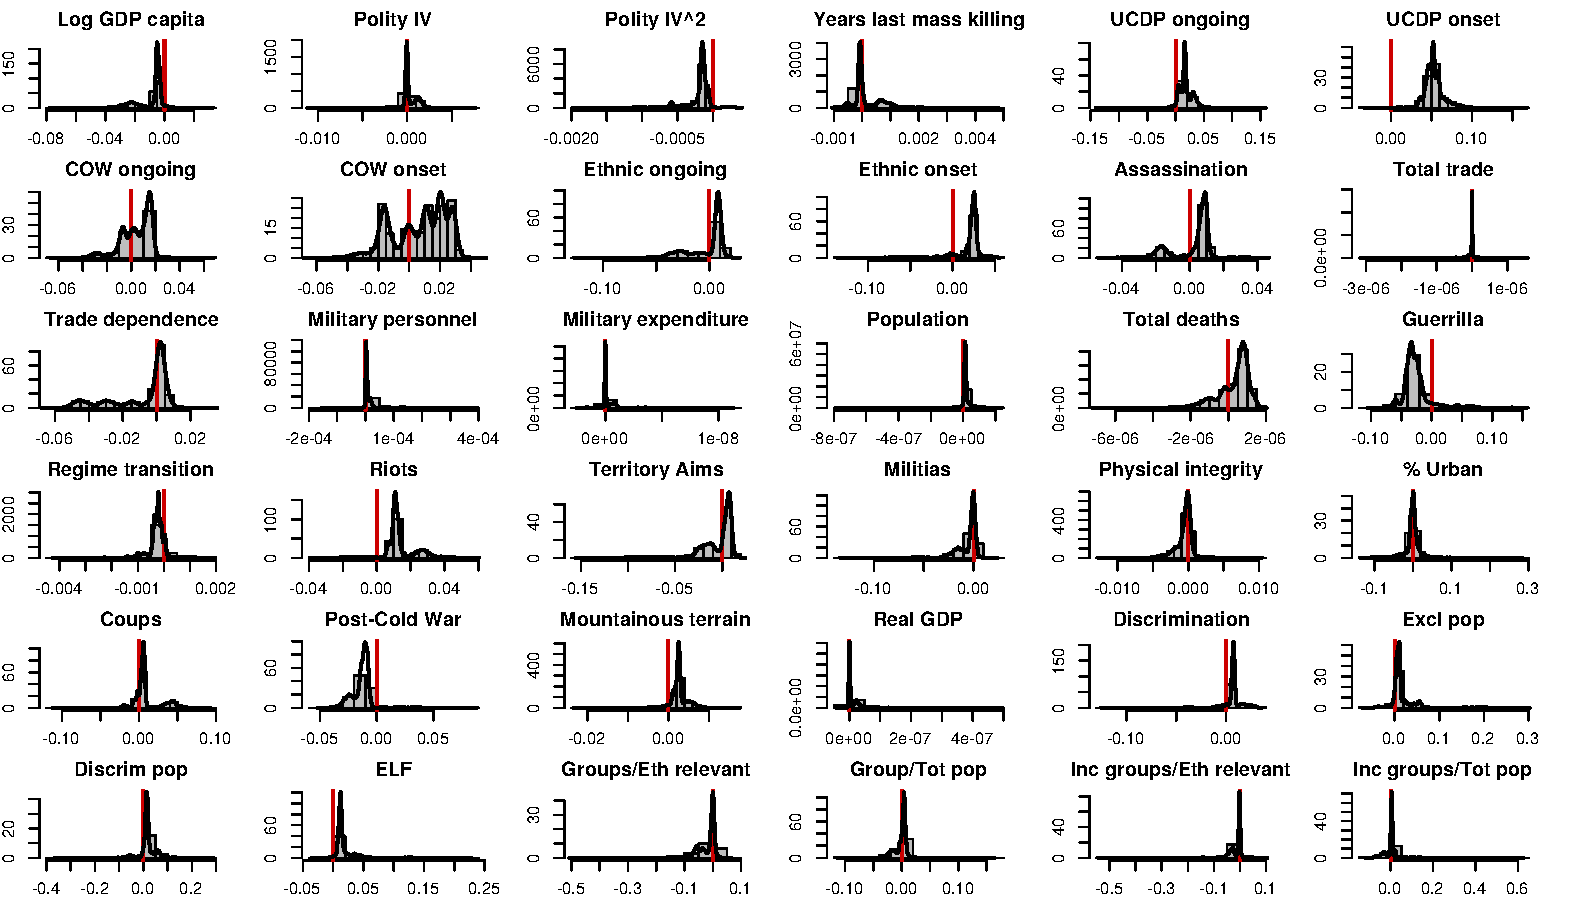
\includegraphics[width=\textwidth]{images/mk.pdf}
    \caption{Extreme Bounds Analysis -- Mass Killings}
    \label{fig:mk}
\end{sidewaysfigure}
\clearpage

\subsubsection{Genocides during Civil Wars}
\label{sec:civil-wars}

Next, we discuss genocides that occur during wartime. We use three covariates that denote ongoing civil conflicts: one by the Uppsala Conflict Data Program \citep{allansson2017organized,gleditsch2002armed}, another by the Correlates of War \citep{sarkees2010resort}, and a third indicating the onset of ethnic conflict as coded by \citet{cederman2010ethnic}. The variables that reach significance in this set of models below are notably different from those obtained in the main estimation. This result provides evidence that mass violence during wartime time follows a separate logic from state killings in peacetime.

\vspace{1cm}

\begin{table}[H]
\centering
\begin{tabular}{lrrrrr}
\hline
\textbf{Variable} & \textbf{Avg. $\beta$} & \textbf{Avg. SE} & \textbf{$\%$ Sig.} & \textbf{CDF(0)} & \textbf{Models} \\ \hline
\textit{UCDP data} &  &  &  &  &  \\
Territory aims & -0.044 & 0.019 & 74.997 & 0.9804 & 17902 \\
Post-Cold War years & -0.038 & 0.019 & 66.574 & 0.9222 & 17902 \\
 &  &  &  &  &  \\
\textit{COW data} &  &  &  &  &  \\
Physical integrity & 0.024 & 0.013 & 66.674 & 0.9564 & 17902 \\
Militias & -0.099 & 0.048 & 73.104 & 0.9490 & 17902 \\
Years since last mass killing & 0.006 & 0.002 & 88.208 & 0.9472 & 101583 \\
Previous riots & 0.078 & 0.041 & 65.412 & 0.9348 & 17902 \\
Ethnic diversity (ELF) & 0.095 & 0.062 & 48.615 & 0.9000 & 17902 \\
 &  &  &  &  &  \\
\textit{Cederman et al. data} &  &  &  &  &  \\
Territory aims & -0.051 & 0.026 & 74.288 & 0.9167 & 17902 \\
Militias & -0.050 & 0.035 & 52.240 & 0.9101 & 17902 \\ \hline
\end{tabular}
\caption{EBA -- Mass Killings during Civil Wars}
\label{tab:ucdp1}
\end{table}

\clearpage
\begin{sidewaysfigure}
    \centering
    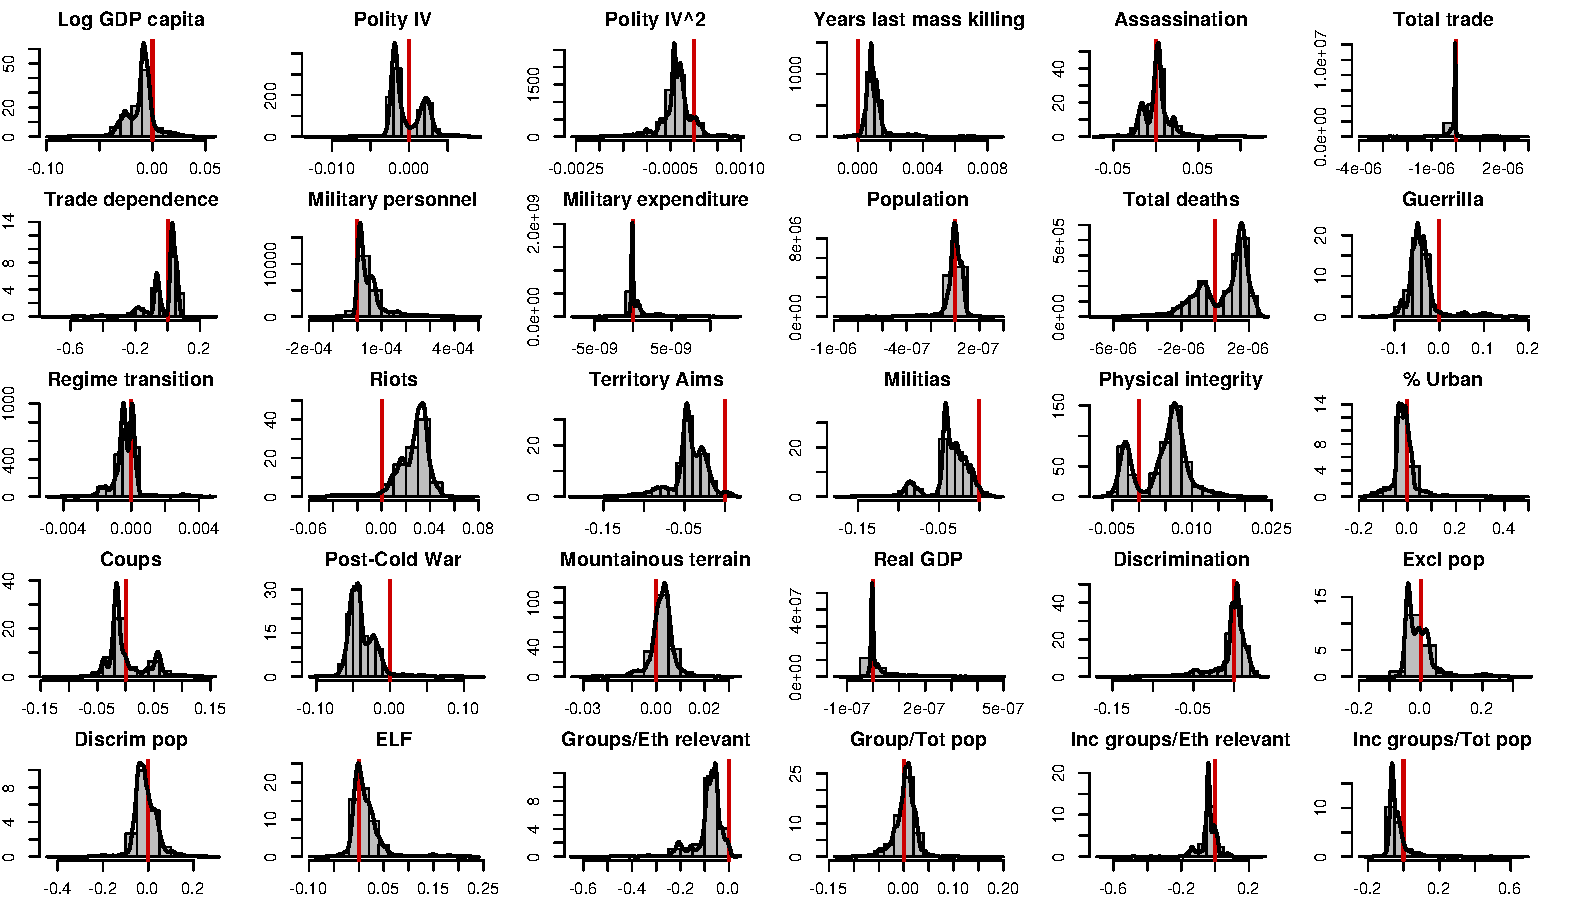
\includegraphics[width=\textwidth]{images/mk-ucdp.pdf}
    \caption{EBA -- Mass Killings during Civil Wars (UCDP Data)}
    \label{fig:mk-ucdp}
\end{sidewaysfigure}
\clearpage

\clearpage
\begin{sidewaysfigure}
    \centering
    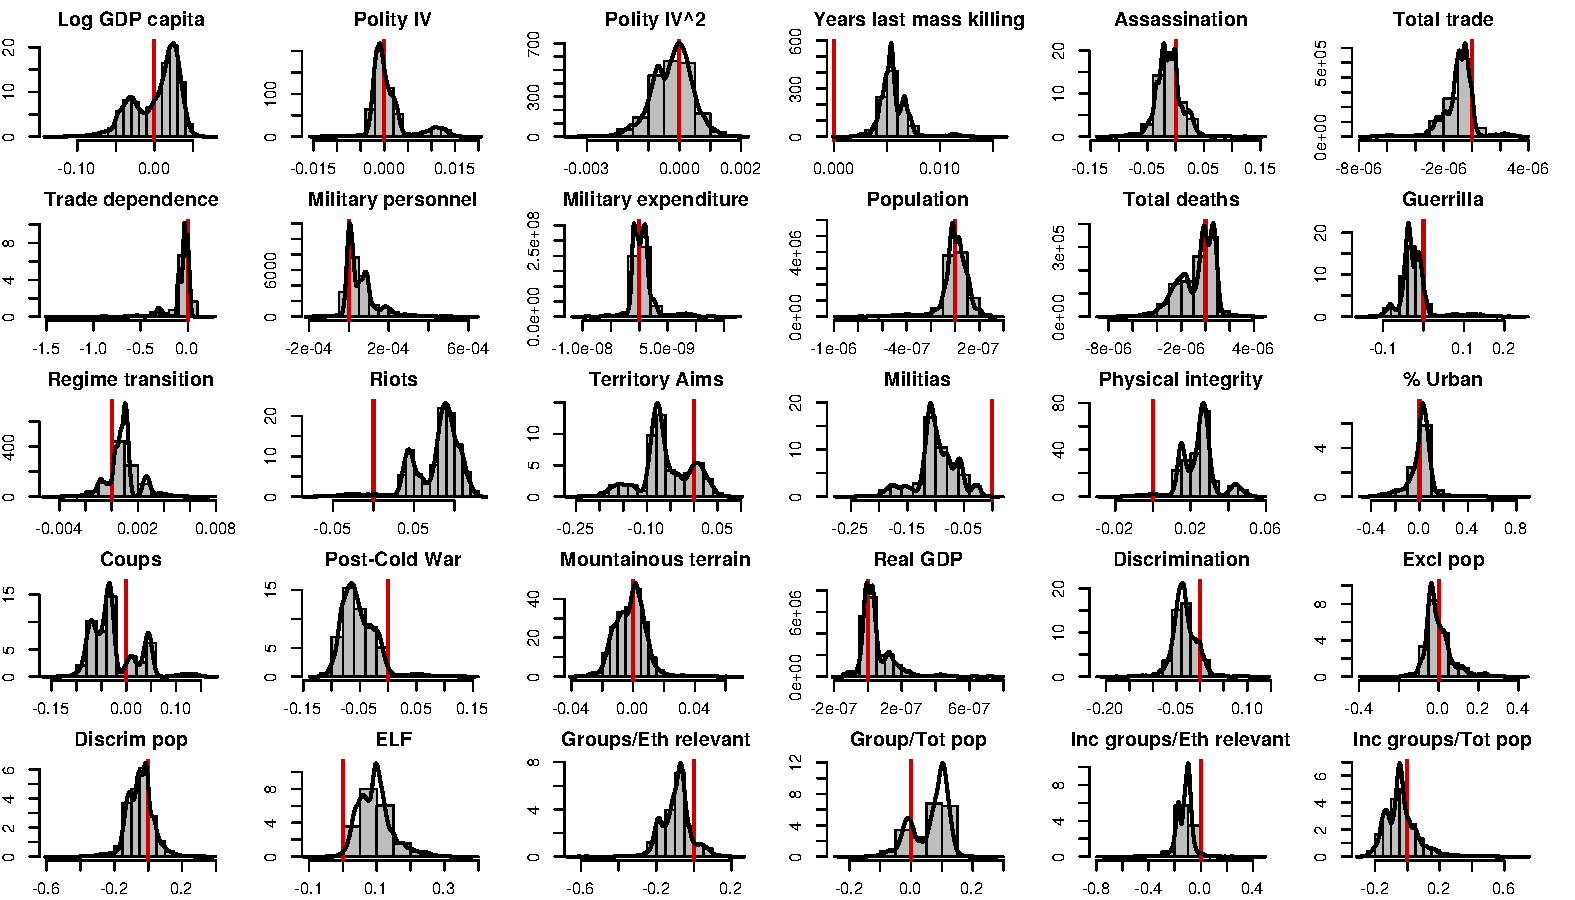
\includegraphics[width=\textwidth]{images/mk-cow.pdf}
    \caption{EBA -- Mass Killings during Civil Wars (COW Data)}
    \label{fig:mk-cow}
\end{sidewaysfigure}
\clearpage

\clearpage
\begin{sidewaysfigure}
    \centering
    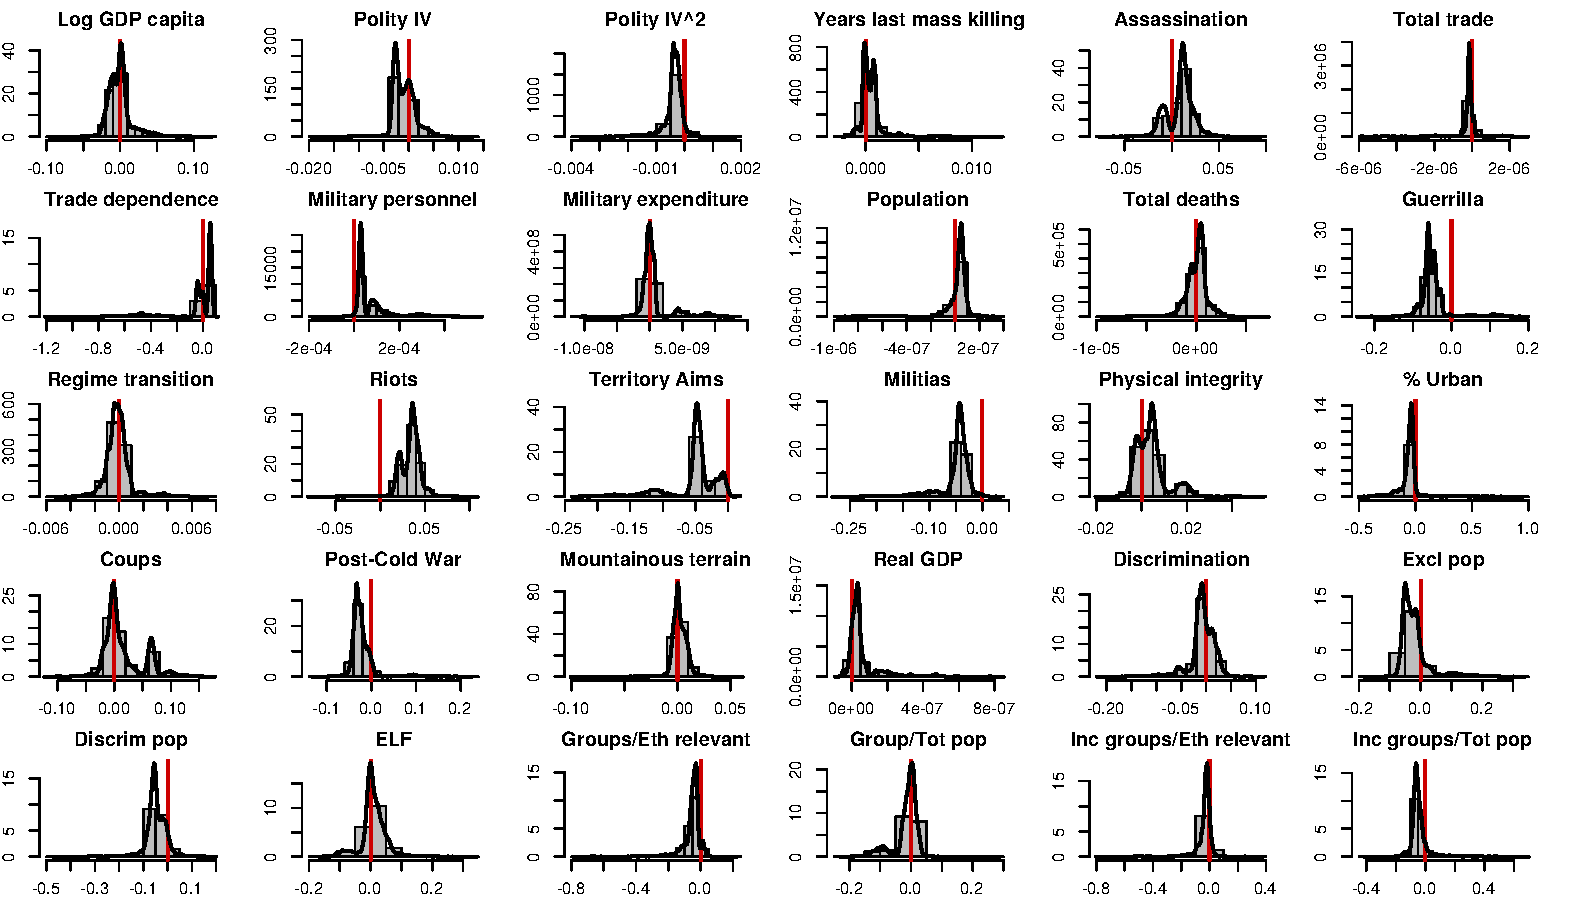
\includegraphics[width=\textwidth]{images/mk-eth.pdf}
    \caption{EBA -- Mass Killings during ethnic civil wars (Cederman et al. Data)}
    \label{fig:mk-eth}
\end{sidewaysfigure}
\clearpage

\subsubsection{Alternative Number of Variables}

The models below are based on 50,000 random draws from the full set of all possible regression models. \citet[819]{salaimartin2004determinants} argue that random sampling produces unbiased estimates of the regression coefficients with low computational time. The models presented in the article, however, include the full set of possible regressions.

The following table shows the results of an EBA with 3 variable combinations per model. The results are very similar to those reported above.

\vspace{1cm}

\begin{table}[H]
\centering
\begin{tabular}{lrrrrr}
\hline
\textbf{Variable} & \textbf{Avg. $\beta$} & \textbf{Avg. SE} & \textbf{$\%$ Sig.} & \textbf{CDF(0)} & \textbf{Models} \\ \hline
\textit{Base variables} &  &  &  &  &  \\
Log GDP per capita & 0.0082 & 0.0043 & 81.439 & 0.9504 & 40677 \\
 &  &  &  &  &  \\
\textit{Additional variables} &  &  &  &  &  \\
Post-Cold War years & -0.0121 & 0.0069 & 77.804 & 0.9609 & 5064 \\
UCDP civil war onset & 0.0523 & 0.0292 & 62.561 & 0.9574 & 3304 \\
Previous riots &0.0134 & 0.0084 & 65.936 & 0.9401 & 5064 \\
UCDP ongoing civil war & 0.0177 & 0.0094 & 72.367 & 0.9372 & 3304 \\
Polity IV squared & -0.0002 & 0.0001 & 66.035 & 0.9268 & 5064 \\ 
Ethnic diversity (ELF) & 0.0162 & 0.0110 & 70.794 & 0.9266 & 5064 \\\hline
\end{tabular}
\caption{EBA -- 3 Variables}
\label{tab:mk-3vars}
\end{table}

\clearpage
\begin{sidewaysfigure}
    \centering
    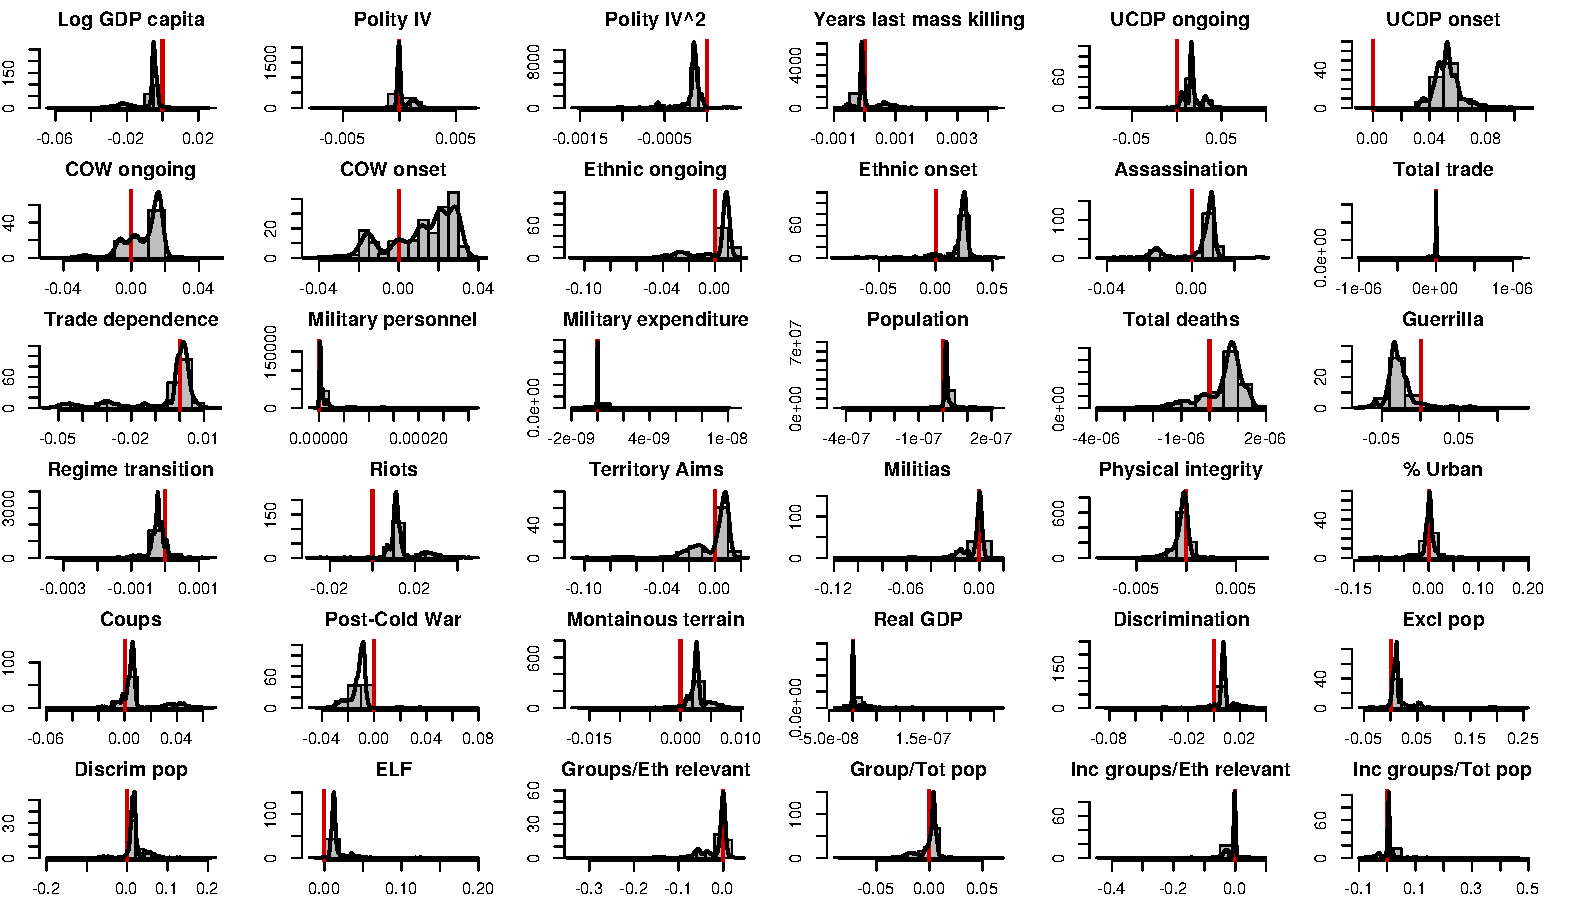
\includegraphics[width=\textwidth]{images/mk-3vars.pdf}
    \caption{EBA -- 3 Variables}
    \label{fig:mk-3vars}
\end{sidewaysfigure}
\clearpage

Table \ref{tab:mk-5vars} presents the results for models with up 5 variables in each regressions. In contrast with our main EBA model, the indicators of UCDP ongoing civil wars, ethnic diversity, and Polity IV square drop out of significance. Their individual CDFs(0) are about 0.88, just marginally below our specified threshold of 0.9.

\vspace{1cm}

\begin{table}[!htpb]
\centering
\begin{tabular}{lrrrrr}
\hline
\textbf{Variable} & \textbf{Avg. $\beta$} & \textbf{Avg. SE} & \textbf{$\%$ Sig.} & \textbf{CDF(0)} & \textbf{Models} \\ \hline
\textit{Base variables} &  &  &  &  &  \\
Log GDP per capita & -0.010 & 0.006 & 70.806 & 0.9161 & 50000 \\
 &  &  &  &  &  \\
\textit{Additional variables} &  &  &  &  &  \\
Post-Cold War years & -0.014 & 0.010 & 68.496 & 0.9336 & 9532 \\
UCDP civil war onset & 0.053 & 0.035 & 44.784 & 0.9308 & 5100 \\
Previous riots & 0.015 & 0.012 & 47.988 & 0.9047 & 9569 \\\hline
\end{tabular}
\caption{EBA -- 5 Variables}
\label{tab:mk-5vars}
\end{table}

\clearpage
\begin{sidewaysfigure}
    \centering
    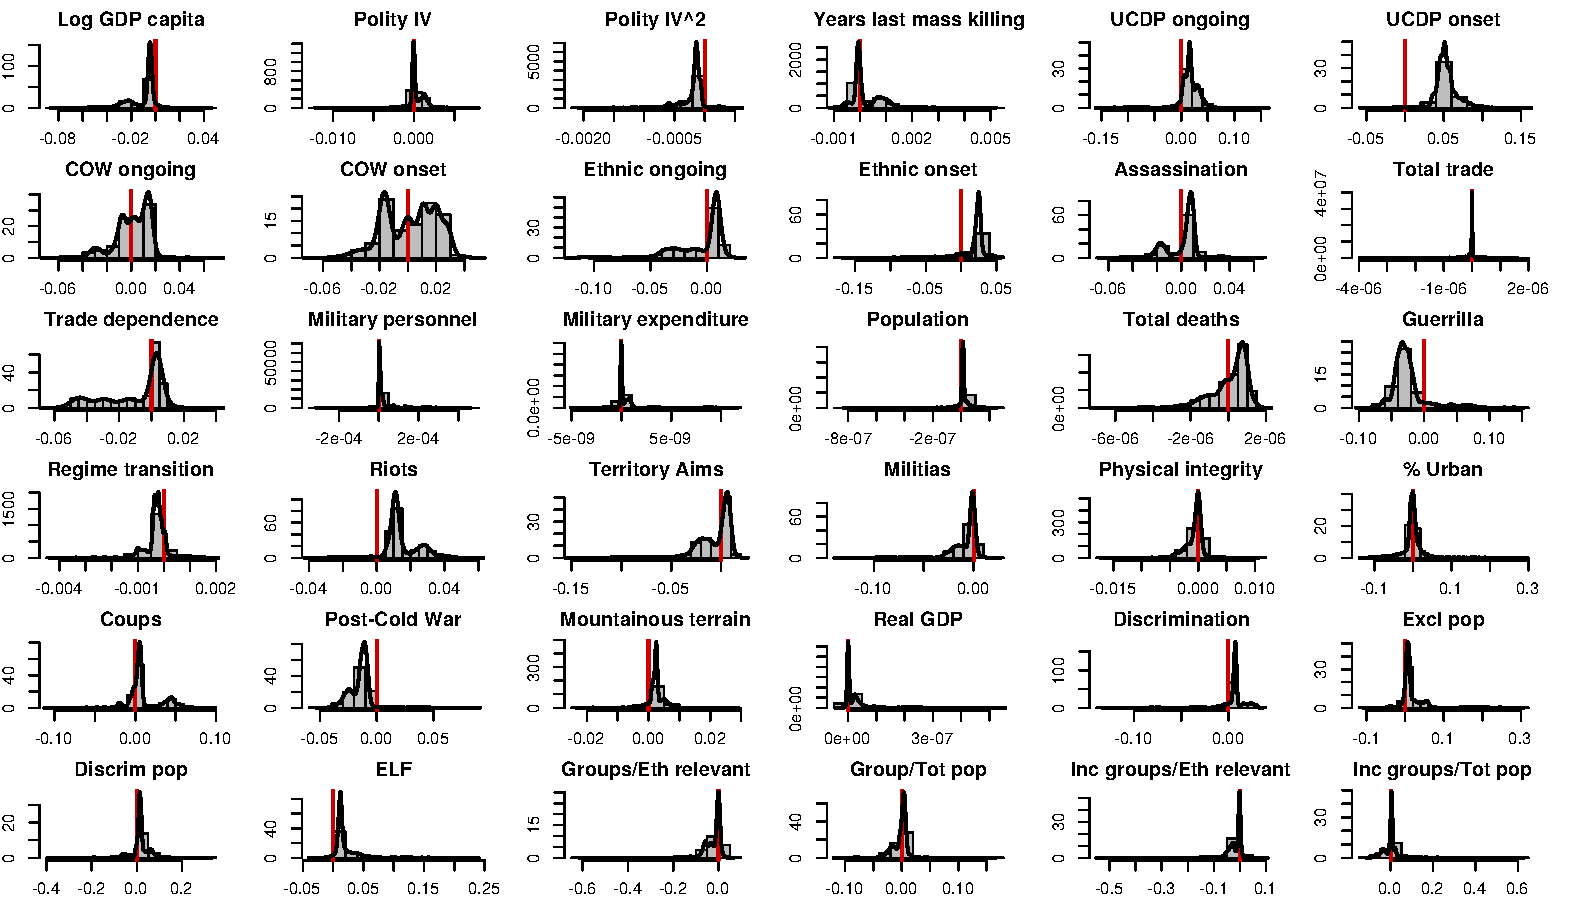
\includegraphics[width=\textwidth]{images/mk-5vars.pdf}
    \caption{EBA -- 5 Variables}
    \label{fig:mk-5vars}
\end{sidewaysfigure}
\clearpage

\subsubsection{Alternative Variance Inflation Factors}

In this subsection, we estimate EBA models with different values of Variance Inflation Factor (VIF), which is a measure of multicollinearity. There is no standard definition about what constitutes an acceptable VIF value, although researchers often use 10 as rule of thumb to indicate strong multicollinearity \citep[674]{o2007caution}. Our original model used a slightly more conservative value of 7 as a cutoff. Here, we test the same model with VIF $=$ 10 (less strict), 2.5 (more conservative), and a model without VIF restrictions. The results are essentially identical to those of the main model. In the model with no VIF restriction, however, ethnic fractionalisation fails to meet the threshold by a very small margin. The CDF(0) of that covariate is 0.897, very close to the required value of 0.9. 

\vspace{1cm}

\begin{table}[H]
\centering
\begin{tabular}{lrrrrr}
\hline
\textbf{Variable} & \textbf{Avg. $\beta$} & \textbf{Avg. SE} & \textbf{$\%$ Sig.} & \textbf{CDF(0)} & \textbf{Models} \\ \hline
\textit{Base variables} &  &  &  &  &  \\
Log GDP per capita & -0.0091 & 0.0052 & 76.354 & 0.9343 & 50000 \\
 &  &  &  &  &  \\
\textit{Additional variables} &  &  &  &  &  \\
Post-Cold War years & -0.0134 & 0.0084 & 73.540 & 0.9495 & 7929 \\
UCDP civil war onset & 0.0529 & 0.0322 & 52.141 & 0.9438 & 4553 \\
Previous riots & 0.0140 & 0.0100 & 56.433 & 0.9216 & 7772 \\
UCDP ongoing civil war & 0.0172 & 0.0113 & 66.013 & 0.9113 & 4587 \\
Ethnic diversity (ELF) & 0.0182 & 0.0136 & 56.872 & 0.9056 & 8076 \\
Polity IV squared & -0.0002 & 0.0001 & 60.791 & 0.9021 & 7835 \\ \hline
\end{tabular}
\caption{EBA -- VIF 10}
\label{tab:mk-high-vif}
\end{table}


\clearpage
\begin{sidewaysfigure}
    \centering
    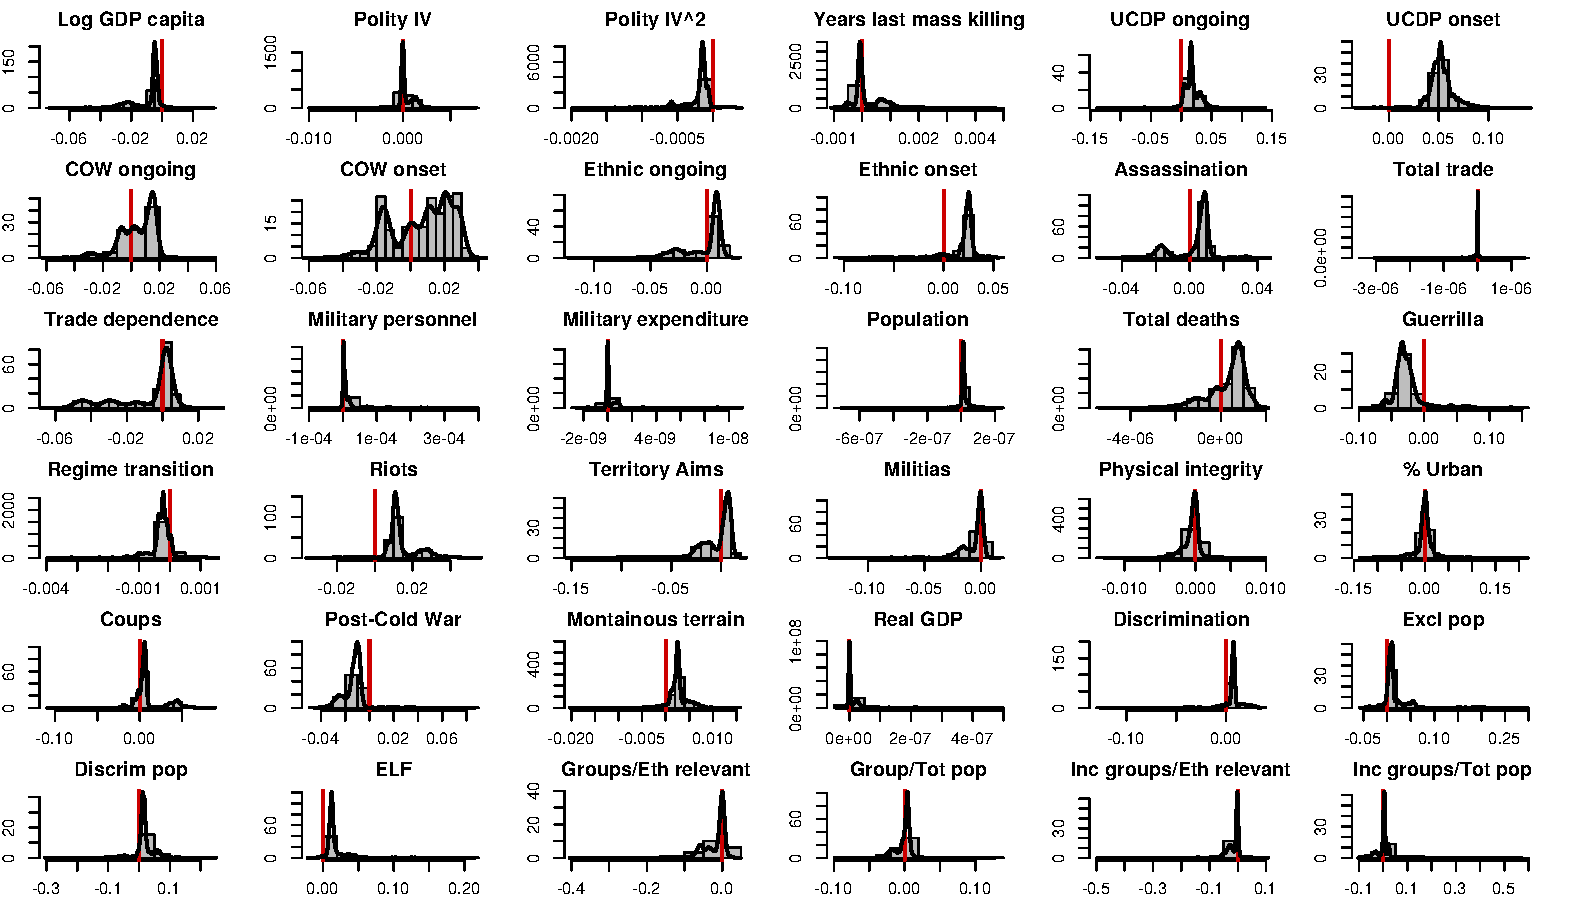
\includegraphics[width=\textwidth]{images/mk-high-vif.pdf}
    \caption{EBA -- VIF 10}
    \label{fig:mk-high-vif}
\end{sidewaysfigure}
\clearpage

\vspace{1cm}

\begin{table}[H]
\centering
\begin{tabular}{lrrrrr}
\hline
\textbf{Variable} & \textbf{Avg. $\beta$} & \textbf{Avg. SE} & \textbf{$\%$ Sig.} & \textbf{CDF(0)} & \textbf{Models} \\ \hline
\textit{Base variables} &  &  &  &  &  \\
Log GDP per capita & -0.0090 & 0.0051 & 76.055 & 0.9343 & 49620 \\
 &  &  &  &  &  \\
\textit{Additional variables} &  &  &  &  &  \\
Post-Cold War years & -0.0132 & 0.0084 & 72.845 & 0.9490 & 7929 \\
UCDP civil war onset & 0.0529 & 0.0322 & 52.378 & 0.9438 & 4553 \\
Previous riots & 0.0141 & 0.0101 & 56.242 & 0.9199 & 7772 \\
UCDP ongoing civil war & 0.0174 & 0.0114 & 65.652 & 0.9103 & 4587 \\
Ethnic diversity (ELF) & 0.0184 & 0.0137 & 56.674 & 0.9054 & 8076 \\
Polity IV squared & -0.0002 & 0.0001 & 61.206 & 0.90267 & 7835 \\ \hline
\end{tabular}
\caption{EBA -- VIF 2.5}
\label{tab:low-vif}
\end{table}

\clearpage
\begin{sidewaysfigure}
    \centering
    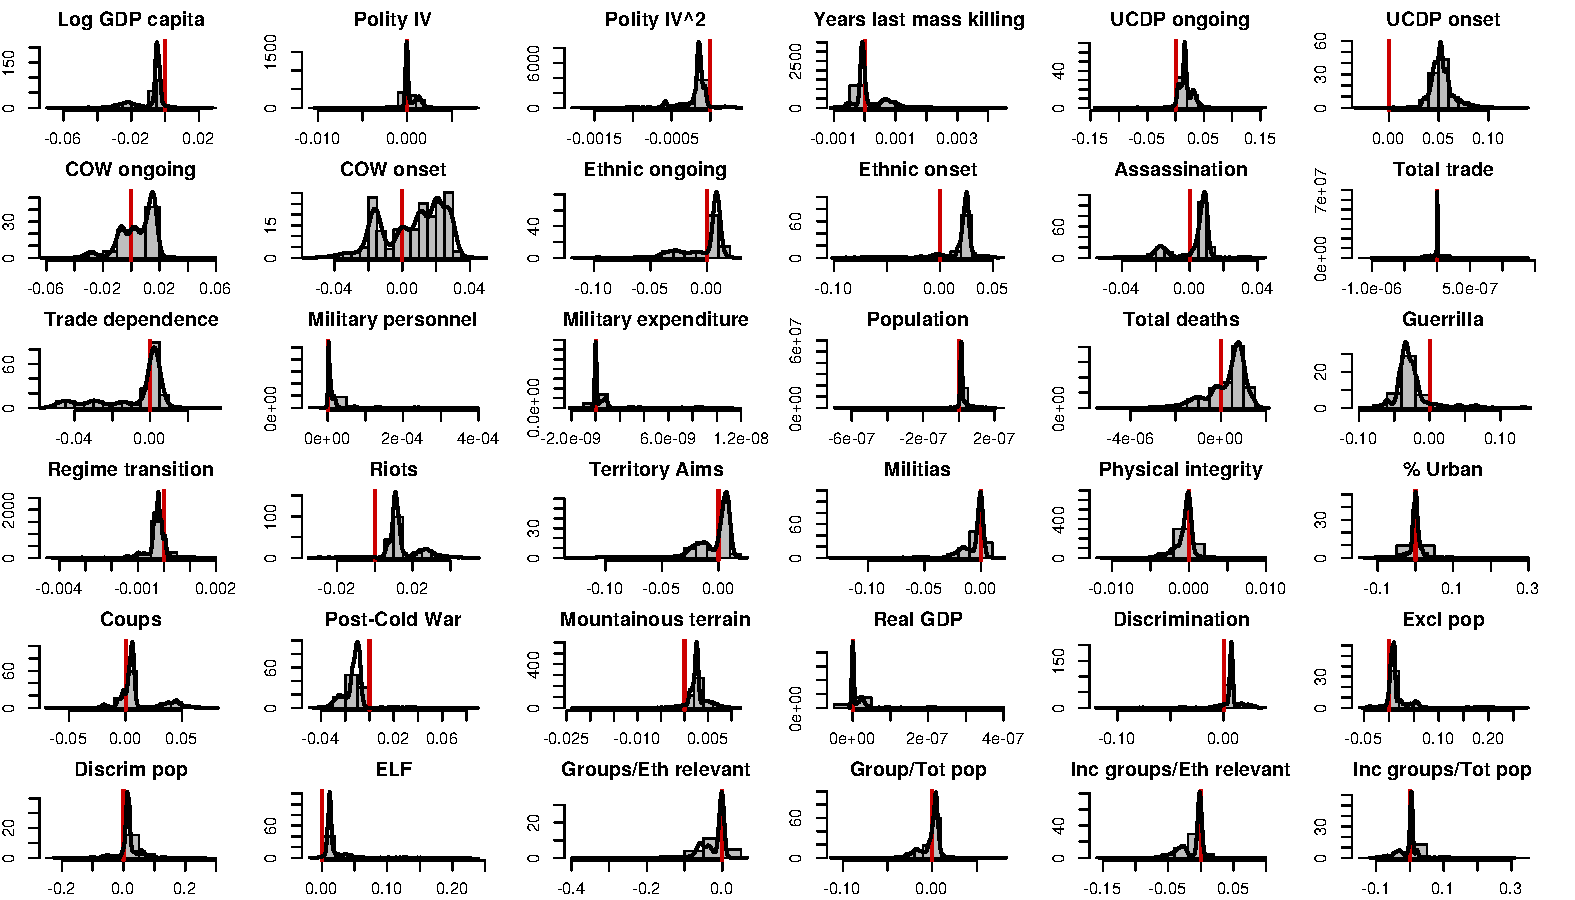
\includegraphics[width=\textwidth]{images/mk-low-vif.pdf}
    \caption{EBA -- VIF 2.5}
    \label{fig:mk-low-vif}
\end{sidewaysfigure}
\clearpage

\begin{table}[H]
\centering
\begin{tabular}{lrrrrr}
\hline
\textbf{Variable} & \textbf{Avg. $\beta$} & \textbf{Avg. SE} & \textbf{$\%$ Sig.} & \textbf{CDF(0)} & \textbf{Models} \\ \hline
\textit{Base variables} &  &  &  &  &  \\
Log GDP per capita & -0.0091 & 0.0052 & 75.940 & 0.9343 & 50000 \\
 &  &  &  &  &  \\
\textit{Additional variables} &  &  &  &  &  \\
Post-Cold War years & -0.0133 & 0.0085 & 72.756 & 0.9469 & 7800 \\
UCDP civil war onset & 0.0531 & 0.0321 & 53.068 & 0.9452 & 4596 \\
Previous riots & 0.0140 & 0.0101 & 56.139 & 0.9200 & 7811 \\
UCDP ongoing civil war & 0.0170 & 0.0116 & 64.487 & 0.9057 & 4497 \\
Ethnic diversity (ELF) & 0.0184 & 0.0137 & 56.814 & 0.9056 & 7808 \\
Polity IV squared & -0.0002 & 0.0001 & 60.825 & 0.9009 & 7903 \\ \hline
\end{tabular}
\caption{EBA -- No VIF Restriction}
\label{tab:mk-no-vif}
\end{table}

\clearpage
\begin{sidewaysfigure}
    \centering
    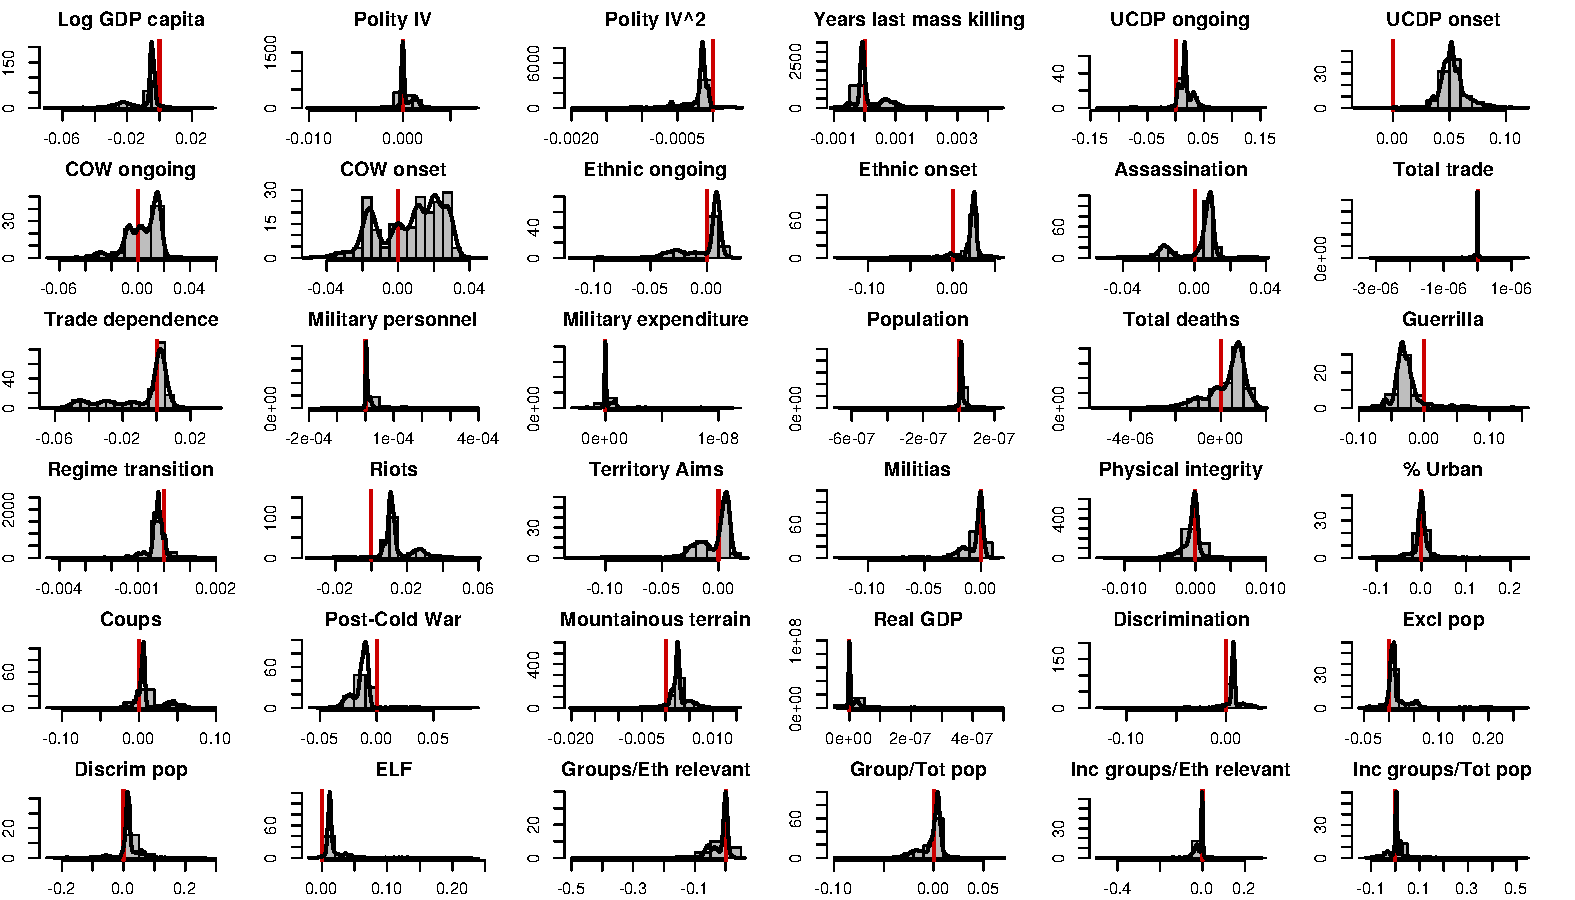
\includegraphics[width=\textwidth]{images/mk-no-vif.pdf}
    \caption{EBA -- No VIF restriction}
    \label{fig:mk-no-vif}
\end{sidewaysfigure}
\clearpage

\subsubsection{Generalised Linear Models}

We reestimate the main EBA model with logit and probit models. Nevertheless, logistic and probit regressions may have issues of complete separation, that is, some covariates may perfectly separate zeros and ones in the outcome variable. In that case, the estimations fail to converge. We address this problem by adding a weak prior to the regression coefficients as suggested by \citet{gelman2008weakly}.\footnote{We thank Mark Bell for sharing \texttt{R} code to estimate penalised-likelihood models.} First, we scaled the non-binary variables to have a mean of 0 and a standard deviation of 0.5, then added a Cauchy distribution with centre 0 and scale 2.5. The probit regressions use a scale of $2.5 \times 1.6$, which is also recommended by the authors \citep{arm2017rpackage}. Ethnic diversity and ongoing civil wars come close to meeting our threshold values (0.88 and 0.84, respectively), and civil war onset (UCDP) has a higher percentage of significant coefficients and a high CDF(0) area than in the linear probability models.

\vspace{1cm}

\begin{table}[H]
\centering
\begin{tabular}{lrrrrr}
\hline
\textbf{Variable} & \textbf{Avg. $\beta$} & \textbf{Avg. SE} & \textbf{$\%$ Sig.} & \textbf{CDF(0)} & \textbf{Models} \\ \hline
\textit{Base variables} &  &  &  &  &  \\
Log GDP per capita & 0.434 & 0.223 & 75.570 & 0.9267 & 50000 \\
 &  &  &  &  &  \\
\textit{Additional variables} &  &  &  &  &  \\
UCDP civil war onset & 1.308 & 0.530 & 87.261 & 0.9742 & 4506 \\
Post-Cold War years & -0.911 & 0.428 & 70.456 & 0.9448 & 7890 \\
Previous riots & 0.744 & 0.38 & 66.778 & 0.9383 & 7805 \\
Polity IV squared & -0.015 & 0.008 & 68.038 & 0.9285 & 7975 \\ \hline
\end{tabular}
\caption{EBA -- Logistic Regression}
\label{tab:mk-logit}
\end{table}

\clearpage
\begin{sidewaysfigure}
    \centering
    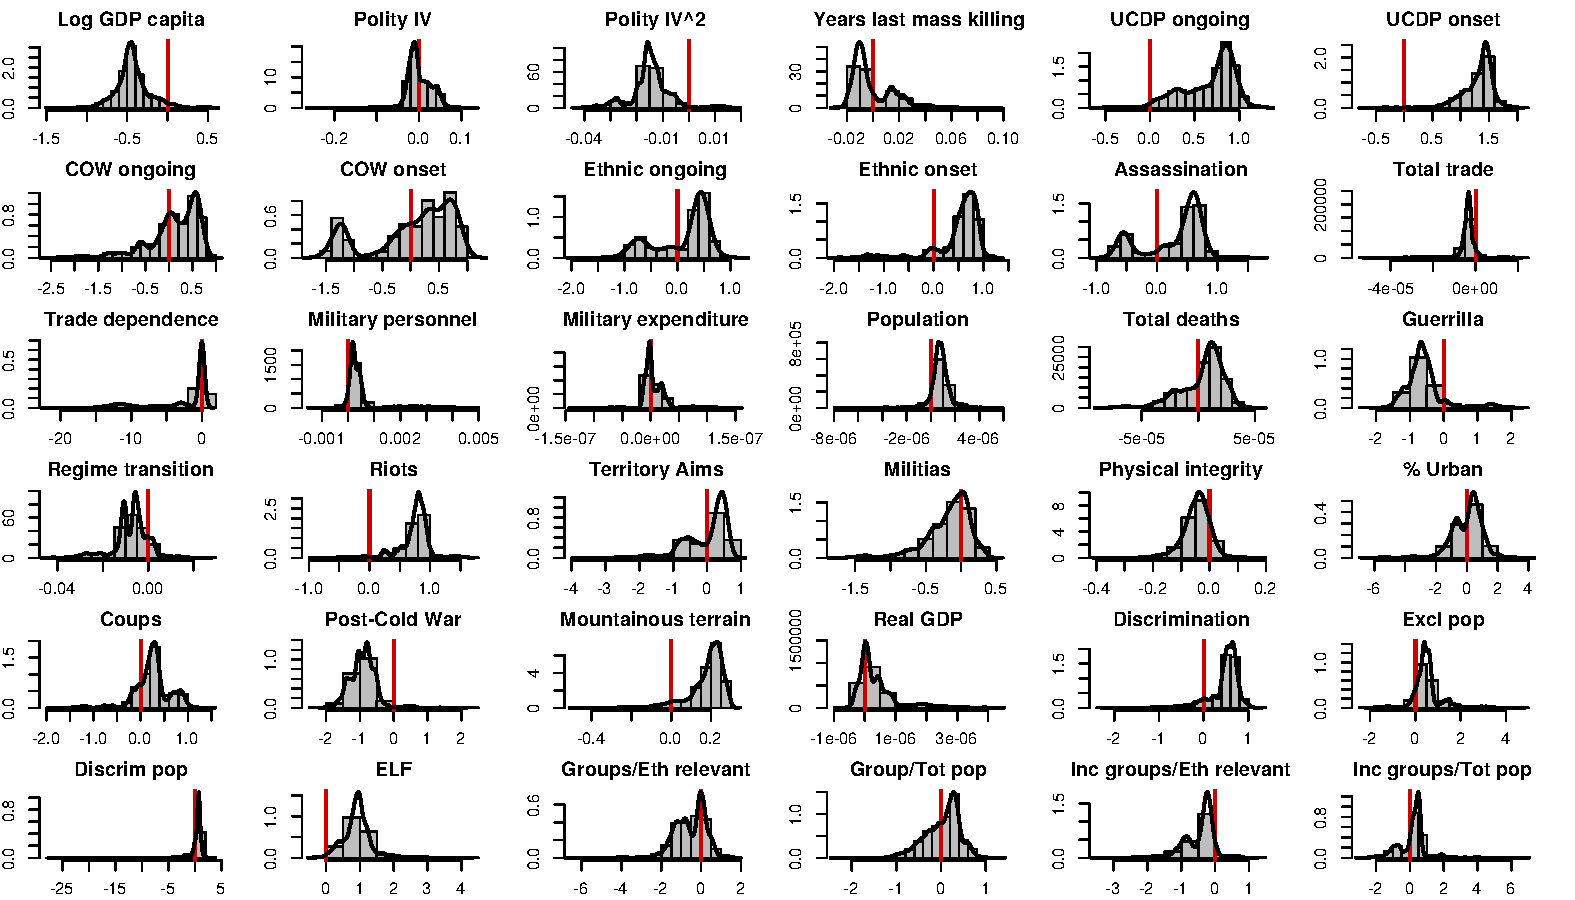
\includegraphics[width=\textwidth]{images/mk-logit.pdf}
    \caption{EBA -- Logistic Regression}
    \label{fig:mk-logit}
\end{sidewaysfigure}
\clearpage

\begin{table}[H]
\centering
\begin{tabular}{lrrrrr}
\hline
\textbf{Variable} & \textbf{Avg. $\beta$} & \textbf{Avg. SE} & \textbf{$\%$ Sig.} & \textbf{CDF(0)} & \textbf{Models} \\ \hline
\textit{Base variables} &  &  &  &  &  \\
Log GDP per capita & -0.1924 & 0.1031 & 76.118 & 0.9258 & 50000 \\
 &  &  &  &  &  \\
\textit{Additional variables} &  &  &  &  &  \\
UCDP civil war onset & 0.6422 & 0.2582 & 89.225 & 0.9772 & 4501 \\
Previous riots & 0.3367 & 0.1743 & 71.813 & 0.9436 & 7851 \\
Post-Cold War years & -0.3709 & 0.1830 & 71.465 & 0.9404 & 7836 \\
Polity IV squared & -0.0061 & 0.0032 & 70.155 & 0.9315 & 7931 \\ \hline
\end{tabular}
\caption{EBA -- Probit Regression}
\label{tab:eba1}
\end{table}

\clearpage
\begin{sidewaysfigure}
    \centering
    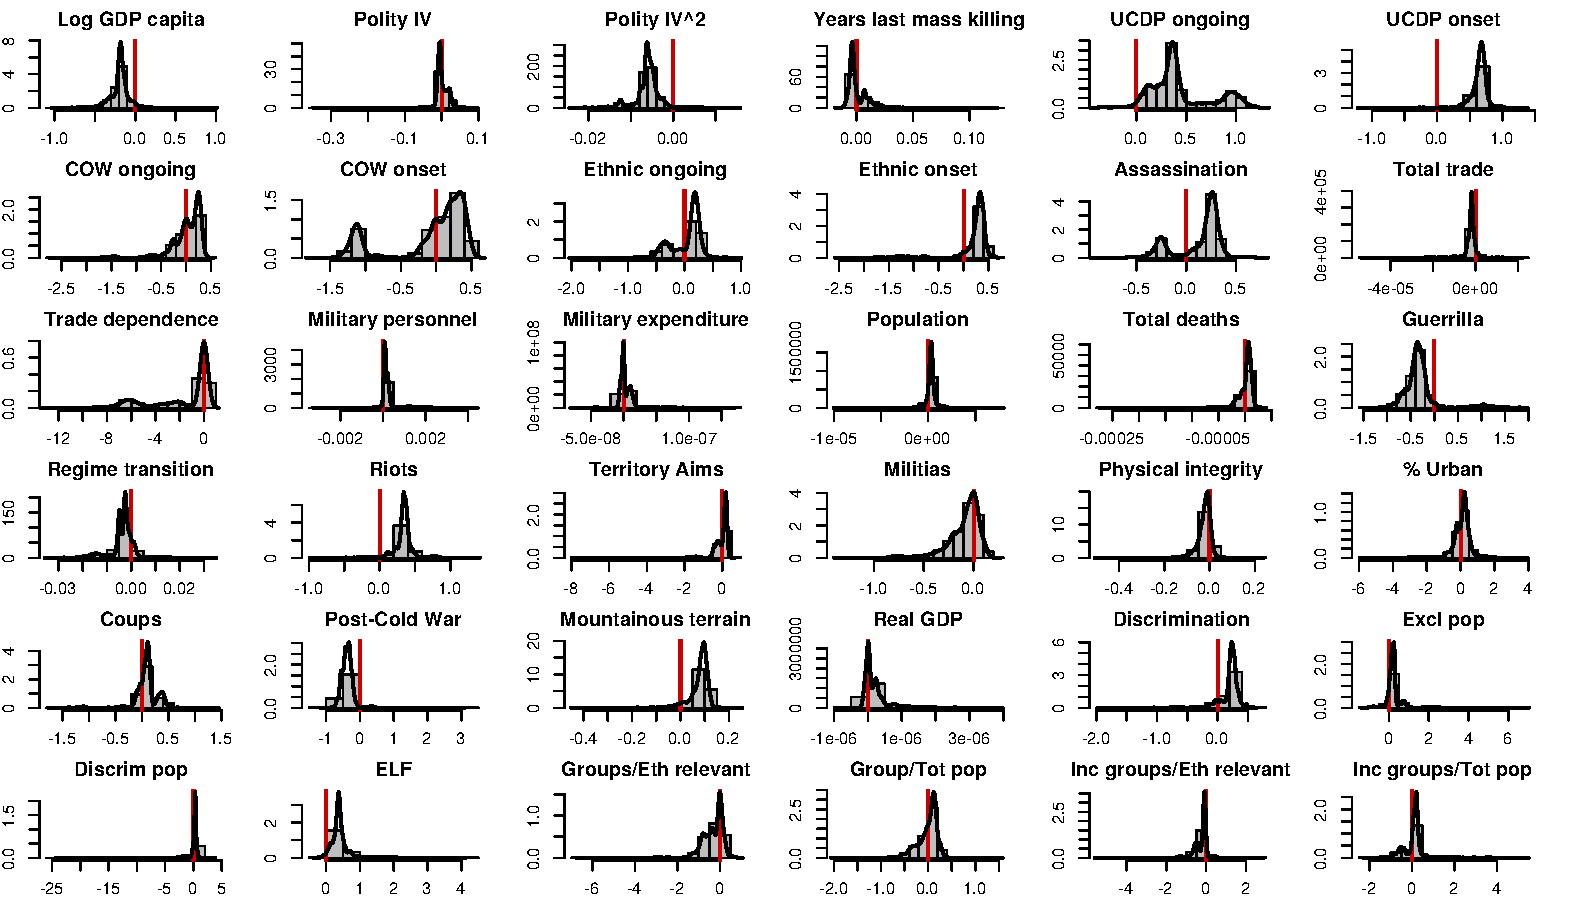
\includegraphics[width=\textwidth]{images/mk-probit.pdf}
    \caption{EBA -- Probit Regression}
    \label{fig:mk-probit}
\end{sidewaysfigure}
\clearpage

\subsection{Random Forest Extensions}
\label{sec:mk-rfe}

\subsubsection{Alternative Random Seeds}

As noted in the article, we perform a grid search to optimise the hyperparameters of the random forest models. The grid search evaluates a wide range of parameter values at once, therefore it is generally unnecessary to run additional tests to assess the robustness of the results. Nevertheless, as random forests themselves are an approximation to a number of possible parameter combinations, changes in seed numbers may influence the output. Thus, we start the models with different random seed numbers to evaluate how sturdy are our original results.\footnote{The numbers were generated at \href{https://www.random.org/}{https://www.random.org/}.} The findings holds quite well: Although variable importance changes from one model to another, the most significant variables appear repeatedly in the estimations. The marginal plots also show that their effects on the outcome variable remains similar despite eventual nonlinearities. We show the six most significant predictors of mass killings and their respective partial dependence plots.

\begin{figure}[H]
    \centering
    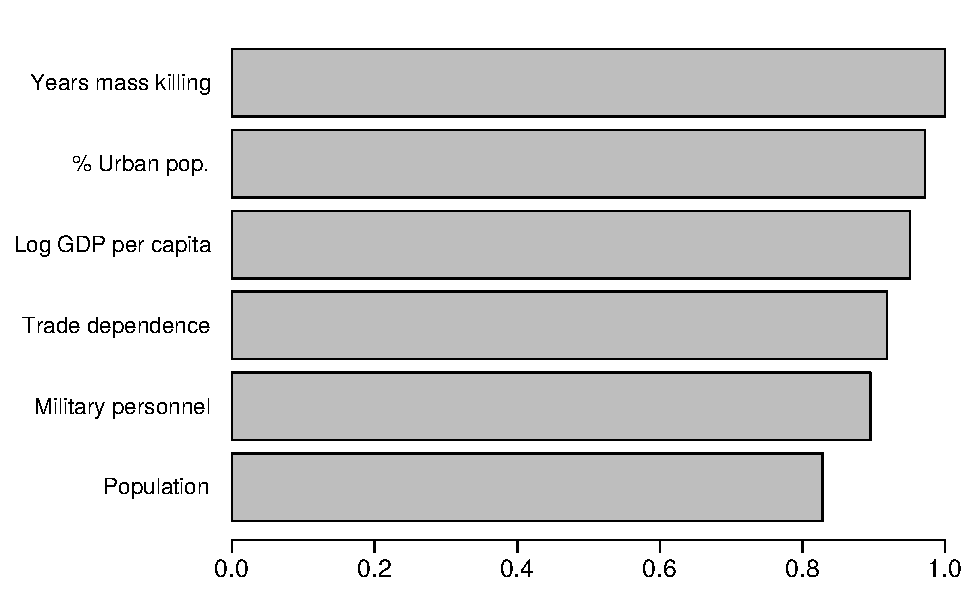
\includegraphics{images/drf-mk2.pdf}
    \caption{Variable Importance -- Seed 44849999}
    \label{fig:my_label}
\end{figure}

\begin{figure}[H]
    \centering
    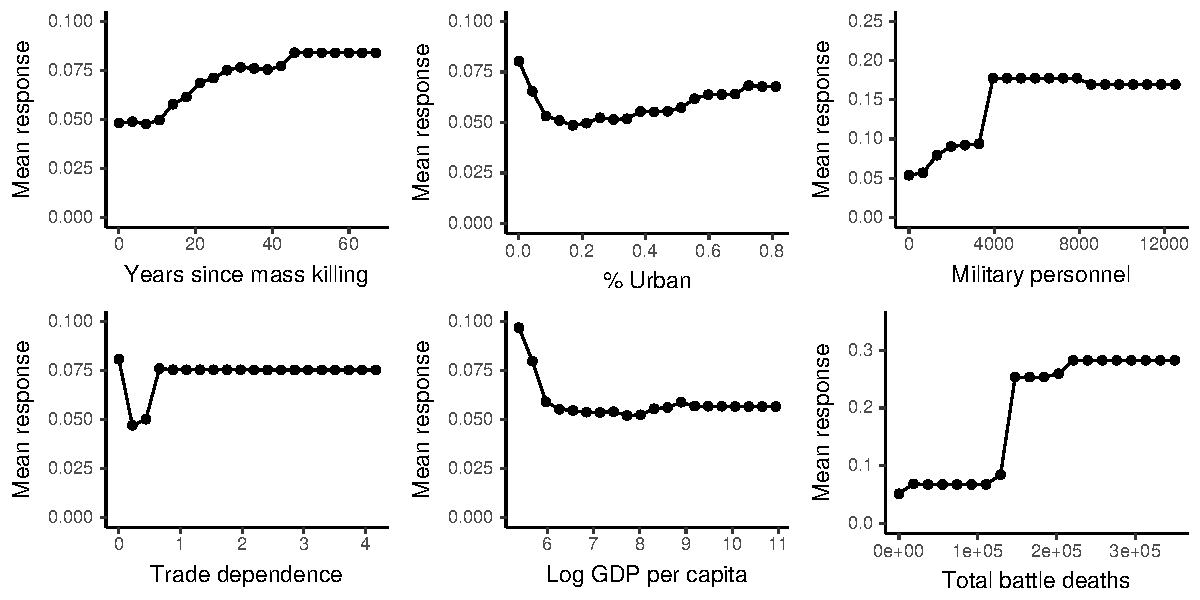
\includegraphics[width=\textwidth, height=9cm]{images/drfdpp2.pdf}
    \caption{Partial Plots -- Seed 44849999}
    \label{fig:my_label}
\end{figure}

\newpage

Second model -- seed 1502436: 

\begin{figure}[H]
    \centering
    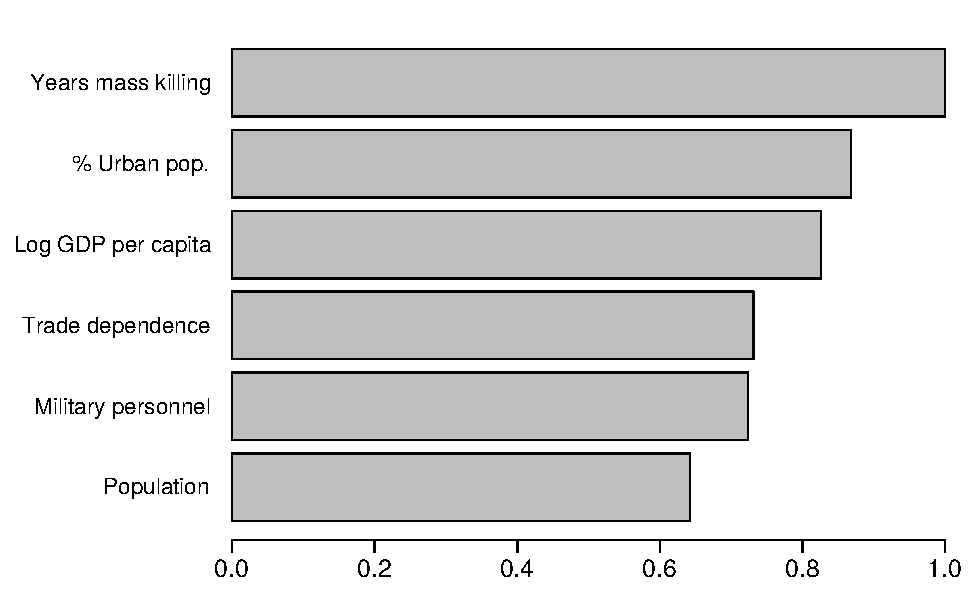
\includegraphics{images/drf-mk3.pdf}
    \caption{Variable Importance -- Seed 1502436}
    \label{fig:my_label}
\end{figure}

\begin{figure}[H]
    \centering
    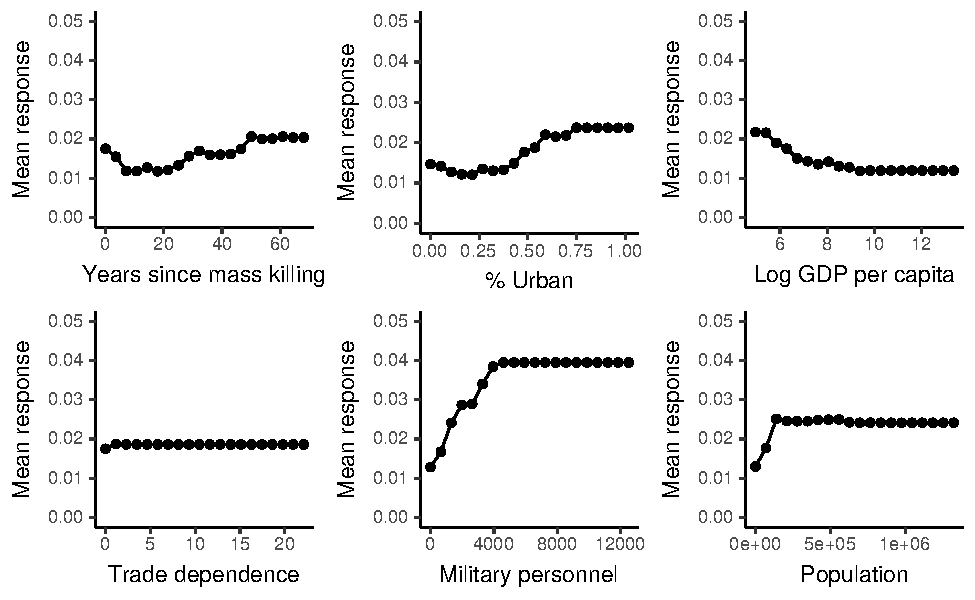
\includegraphics[width=\textwidth, height=9cm]{images/drfdpp3a.pdf}
    \caption{Partial Plots -- Seed 1502436}
    \label{fig:my_label}
\end{figure}

\newpage

\subsection{Genocides/Politicides}
\label{sec:mk-other-variable}

In this section, we evaluate the models presented above with a measure of genocide and politicide by \citet{harff2003no}. The results show important contrasts with the previous analyses. First, no variable appear as significant in the main extreme bounds analysis. That is, none of the 36 predictors reached the threshold of CDF(0) $> 0.9$. The variable that came closest to significance was a dummy indicator of coups d'état, which has a CDF(0) of 0.897 and, as expected, is positively correlated with the onset of genocides. The distribution of the covariates' coefficients are available in figure \ref{fig:uamk}.

\clearpage
\begin{sidewaysfigure}
    \centering
    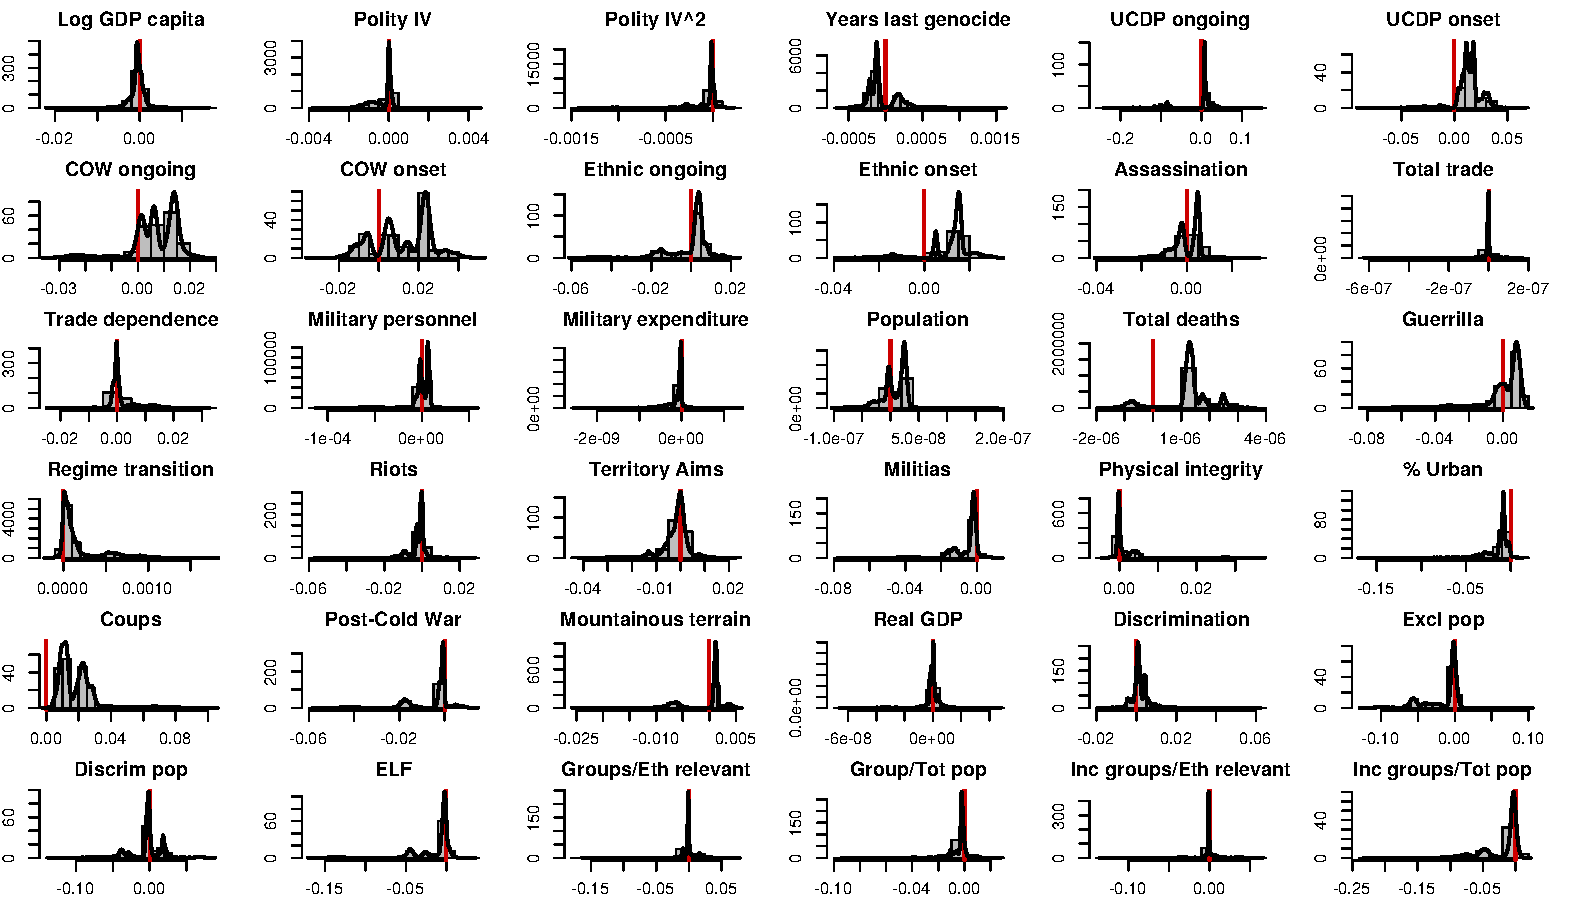
\includegraphics[width=\textwidth]{images/uamk.pdf}
    \caption{EBA -- Genocides/Politicides}
    \label{fig:uamk}
\end{sidewaysfigure}
\clearpage

\subsubsection{Genocides/Politicides during Civil Wars}

Next, we evaluate what covariates are robust when considering only genocides and politicide that occur during civil conflicts. Post-Cold War years again appear as a significant variable and with a negative sign; excluded population also has a negative impact on the outcome variable in two analyses.

\vspace{1cm}

\begin{table}[H]
\centering
\begin{tabular}{lrrrrr}
\hline
\textbf{Variable} & \textbf{Avg. $\beta$} & \textbf{Avg. SE} & \textbf{$\%$ Sig.} & \textbf{CDF(0)} & \textbf{Models} \\ \hline
\textit{UCDP data} &  &  &  &  &  \\
Excluded population & -0.037 & 0.022 & 64.524 & 0.9176 & 8758 \\
 &  &  &  &  &  \\
\textit{COW data} &  &  &  &  &  \\
Excluded population & -0.057 & 0.031 & 65.703 & 0.9570 & 8820 \\
Discriminated population & -0.050 & 0.029 & 53.850 & 0.93.67 & 8767 \\
Post-Cold War years & -0.019 & 0.013 & 42.531 & 0.9203 & 8904 \\
 &  &  &  &  &  \\
\textit{Cederman et al. data} &  &  &  &  &  \\
Assassination dummy & -0.009 & 0.006 & 47.723 & 0.9232 & 8828 \\ \hline
\end{tabular}
\caption{EBA -- Genocides/Politicides}
\label{tab:uamk1}
\end{table}

\newpage
\clearpage
\begin{sidewaysfigure}
    \centering
    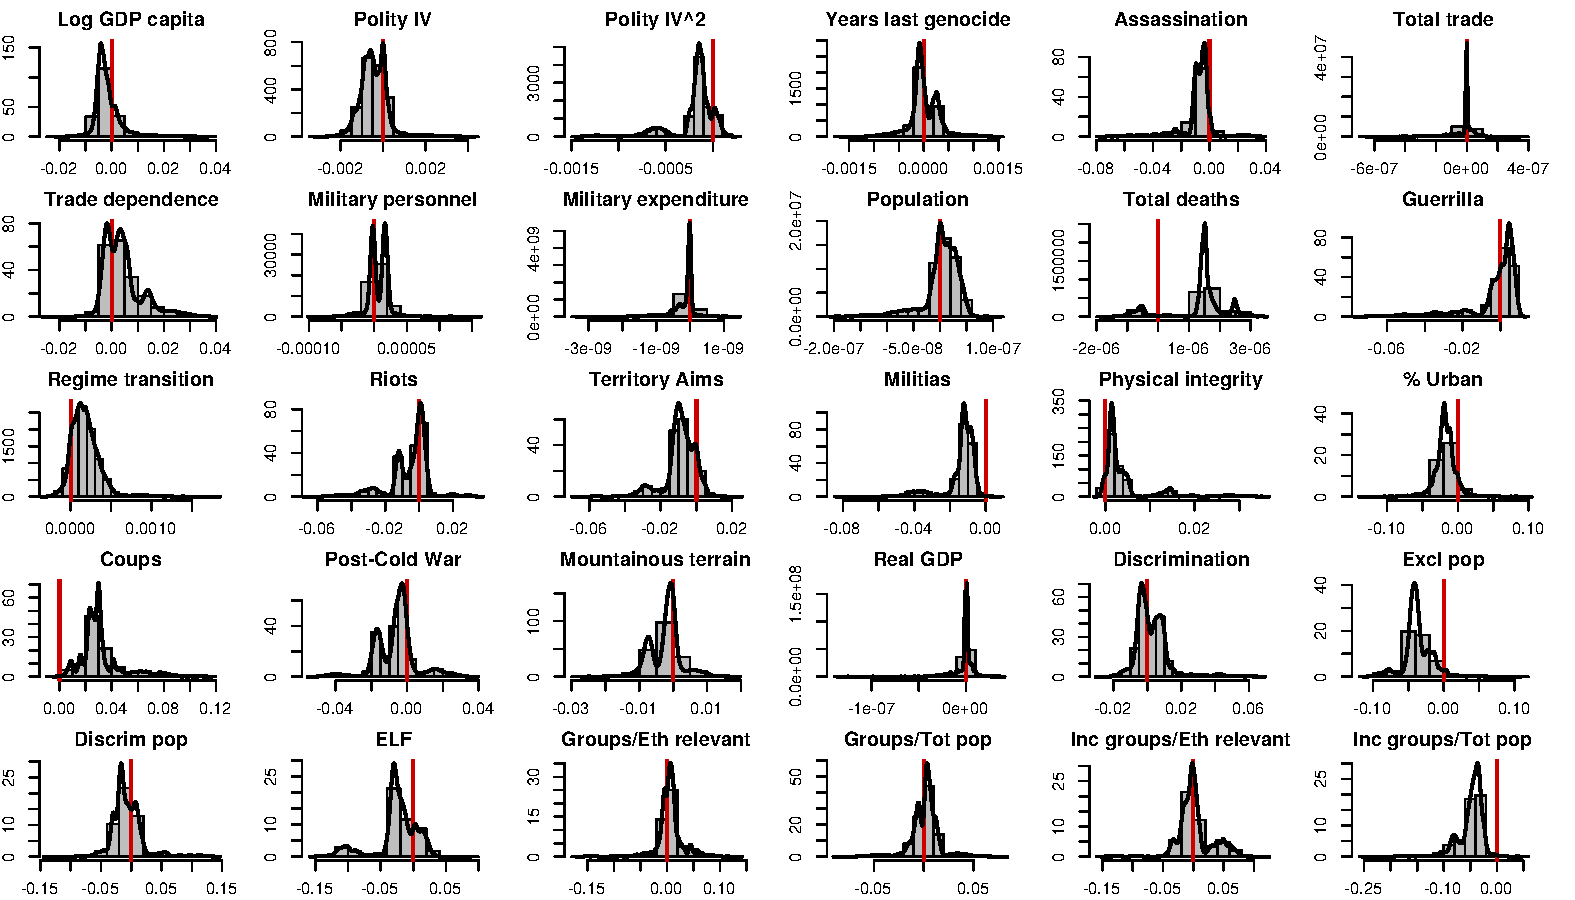
\includegraphics[width=\textwidth]{images/uamk-ucdp.pdf}
    \caption{EBA -- Genocides and Politicides during Civil Wars (UCDP Data)}
    \label{fig:uamk-ucdp}
\end{sidewaysfigure}
\clearpage

\clearpage
\begin{sidewaysfigure}
    \centering
    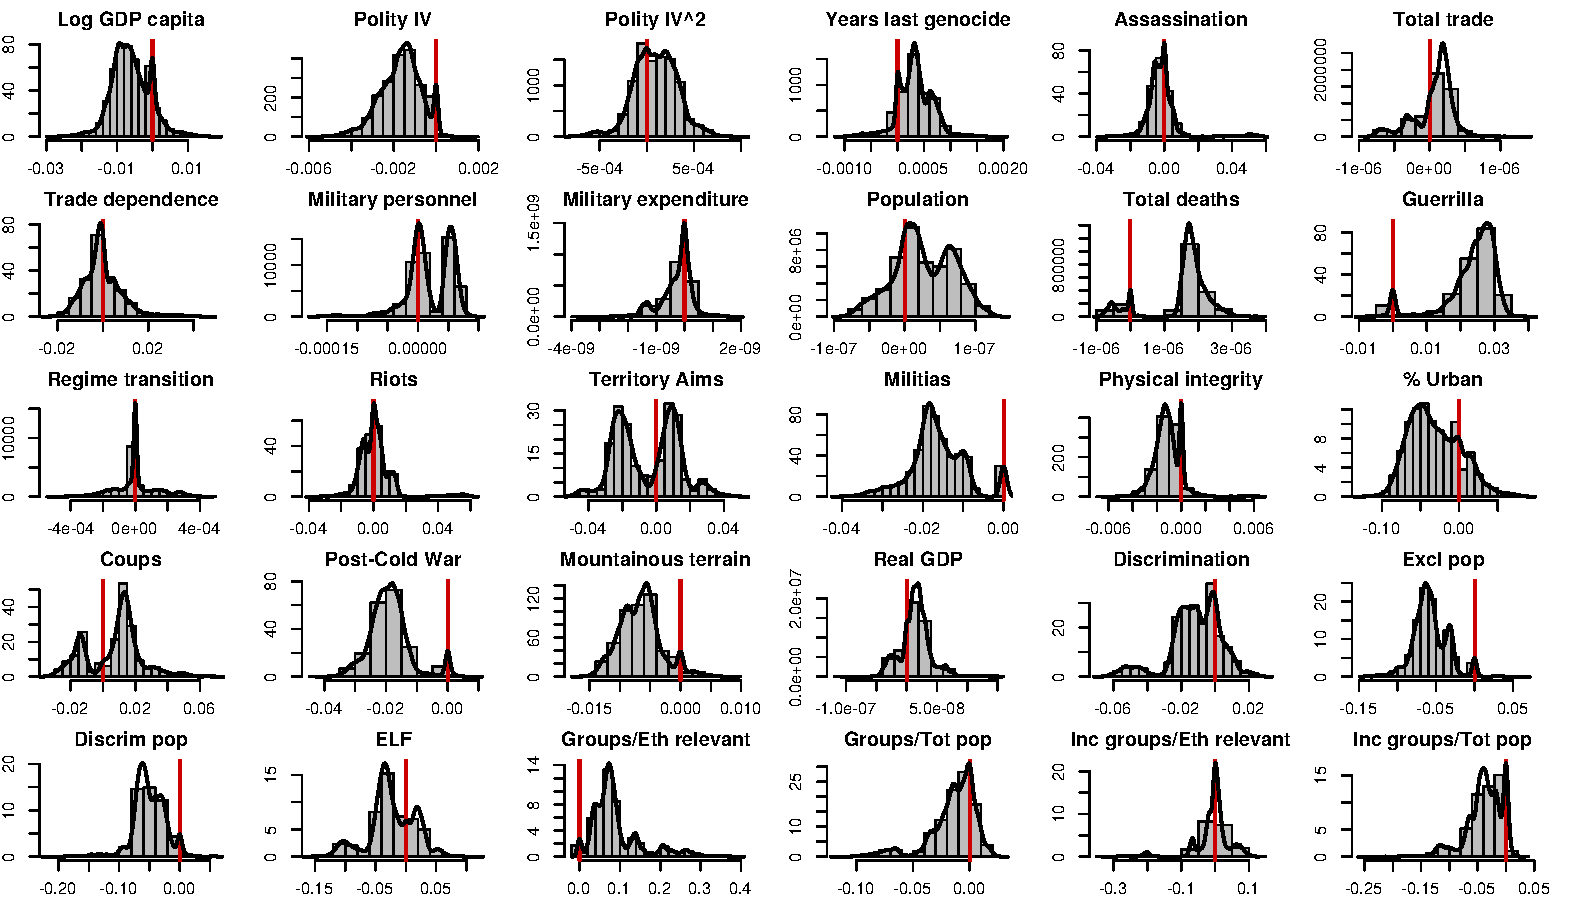
\includegraphics[width=\textwidth]{images/uamk-cow.pdf}
    \caption{EBA -- Genocides and Politicides during Civil Wars (COW Data)}
    \label{fig:uamk-cow}
\end{sidewaysfigure}
\clearpage

\clearpage
\begin{sidewaysfigure}
    \centering
    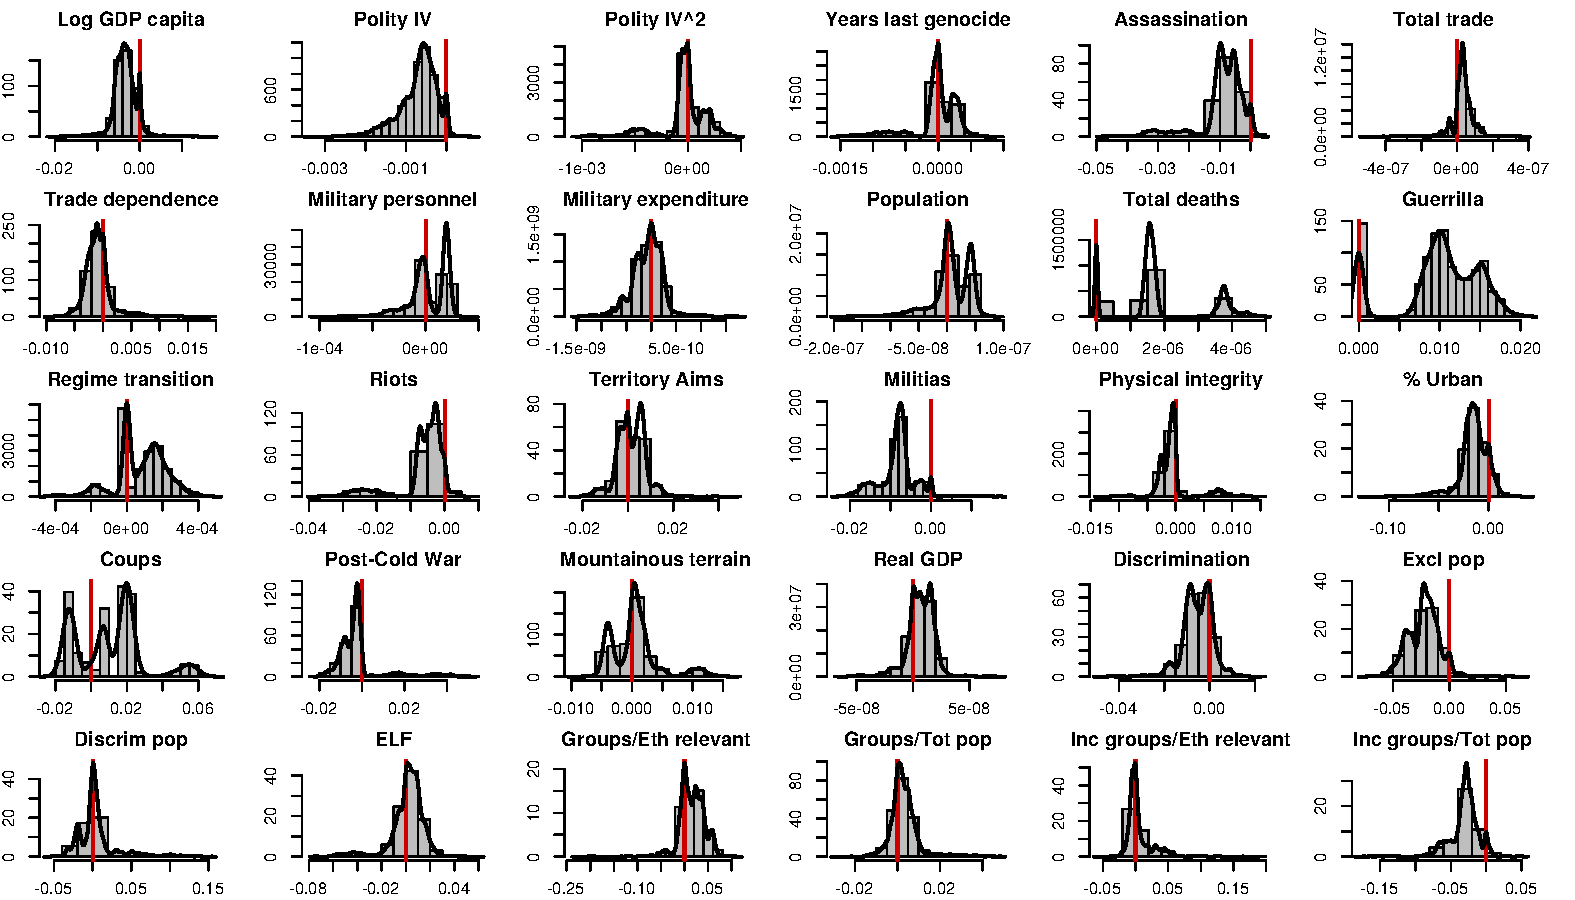
\includegraphics[width=\textwidth]{images/uamk-eth.pdf}
    \caption{EBA -- Genocides and Politicides during Ethnic Civil Wars (Cederman et al. Data)}
    \label{fig:uamk-eth}
\end{sidewaysfigure}
\clearpage

\newpage
\subsection{Genocides/Politicides -- Random Forests}

Lastly, we present three models using the distributed random forest algorithm \citep{h2o2017}. The results are in line with those obtained with the mass killing variable by  \citet{ulfelder2008assessing}. Again, we see that CINC, the percentage of urban population, and variables concerning the military are some of the most important predictors of state-led violence. The results confirm the overall finding of the chapter: Poor countries are more likely to experience mass killings, and states with a stronger army see a significant upward shift in genocide risk.

\begin{figure}[H]
    \centering
    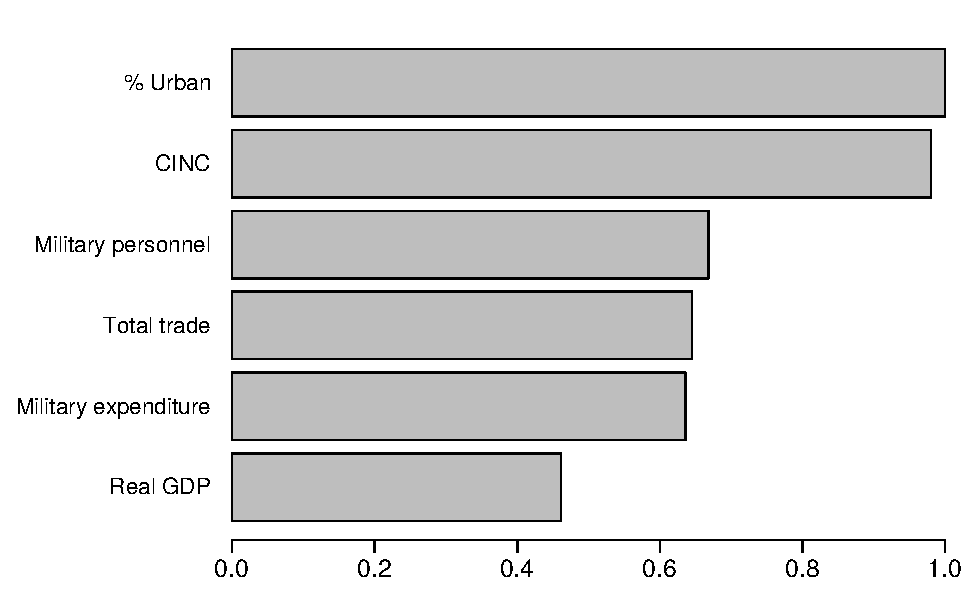
\includegraphics{images/drf-gp.pdf}
    \caption{Variable Importance -- Genocides/Politicides}
    \label{fig:my_label}
\end{figure}

\begin{figure}[H]
    \centering
    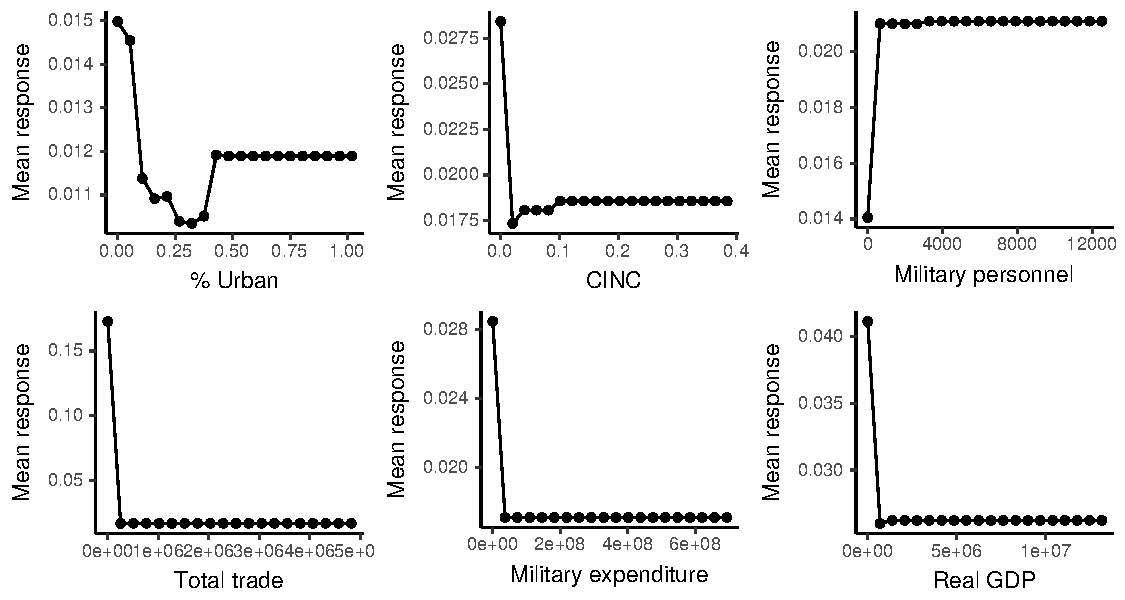
\includegraphics[width=\textwidth, height=9cm]{images/drfdpp4a.pdf}
    \caption{Partial Plots -- Genocides/Politicides}
    \label{fig:my_label}
\end{figure}

\newpage

The next graphs show the most important predictors of genocides that occur during civil wars and their respective partial dependence plots. 

\begin{figure}[H]
    \centering
    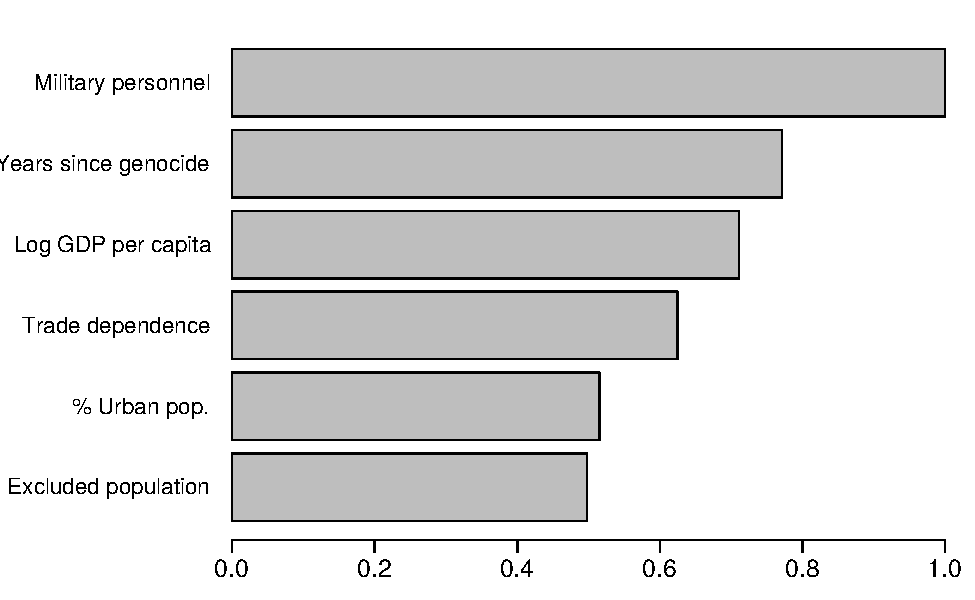
\includegraphics{images/drf-gp1.pdf}
    \caption{Variable Importance -- Genocides/Politicides (UCDP Data)}
    \label{fig:my_label}
\end{figure}

\begin{figure}[H]
    \centering
    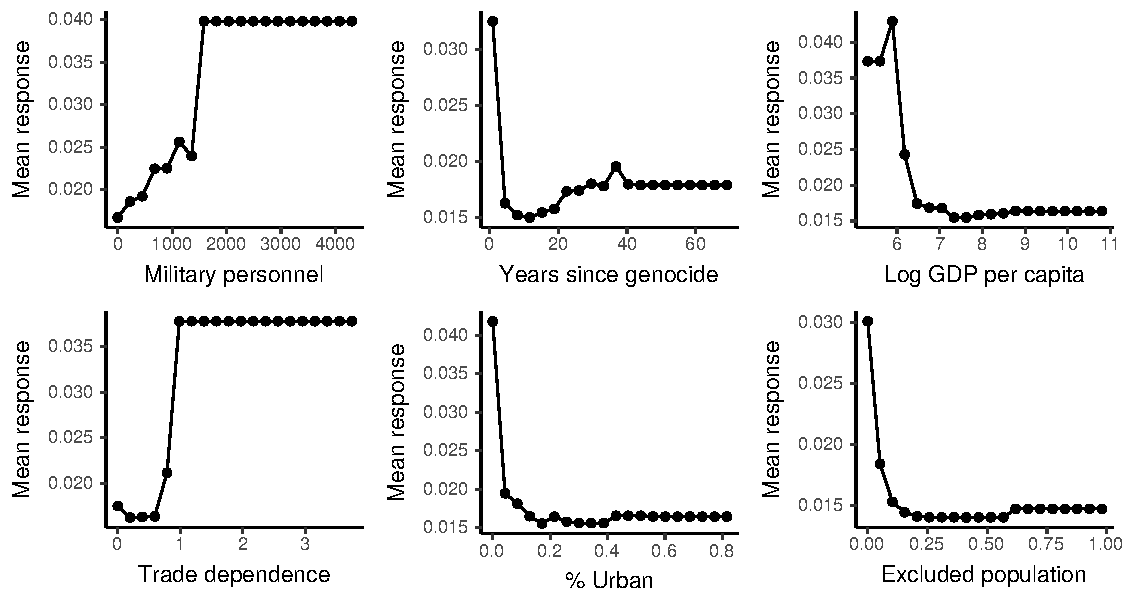
\includegraphics[width=\textwidth, height=9cm]{images/drfdpp5a.pdf}
    \caption{Partial Plots -- Genocides/Politicides (UCDP Data)}
    \label{fig:my_label}
\end{figure}

\begin{figure}[H]
    \centering
    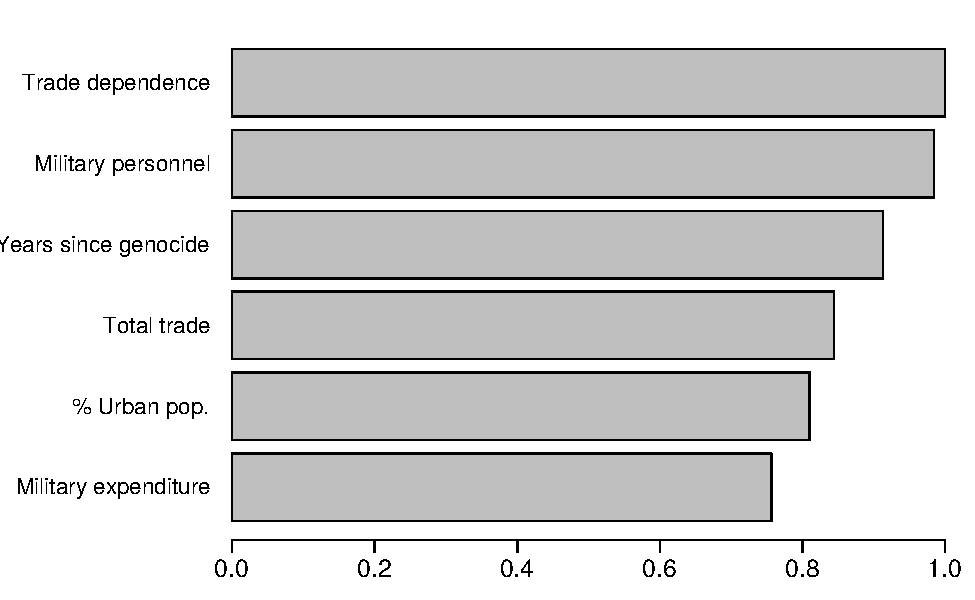
\includegraphics{images/drf-gp2.pdf}
    \caption{Variable Importance -- Genocides/Politicides (COW Data)}
    \label{fig:my_label}
\end{figure}

\begin{figure}[H]
    \centering
    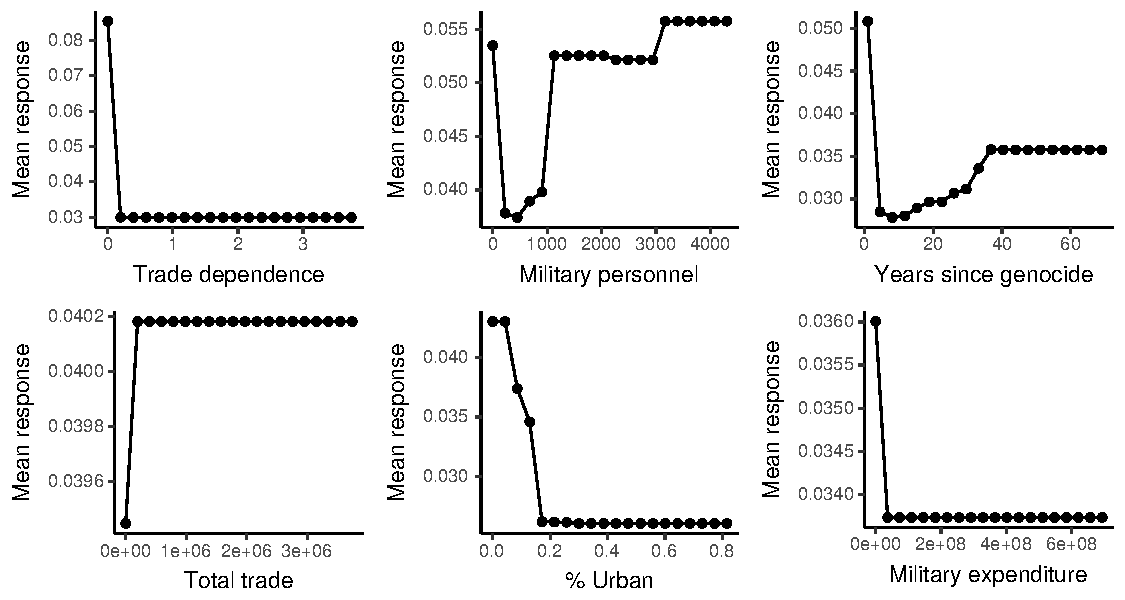
\includegraphics[width=\textwidth, height=9cm]{images/drfdpp6a.pdf}
    \caption{Partial Plots -- Genocides/Politicides (COW Data)}
    \label{fig:my_label}
\end{figure}

\begin{figure}[H]
    \centering
    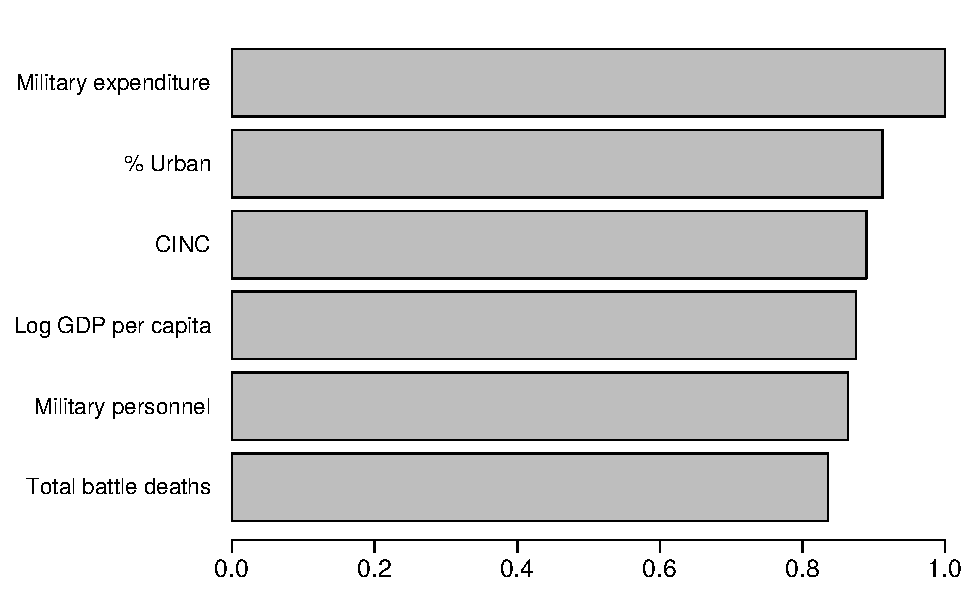
\includegraphics{images/drf-gp3.pdf}
    \caption{Variable Importance -- Genocides/Politicides (Cederman et al. Data)}
    \label{fig:my_label}
\end{figure}

\begin{figure}[H]
    \centering
    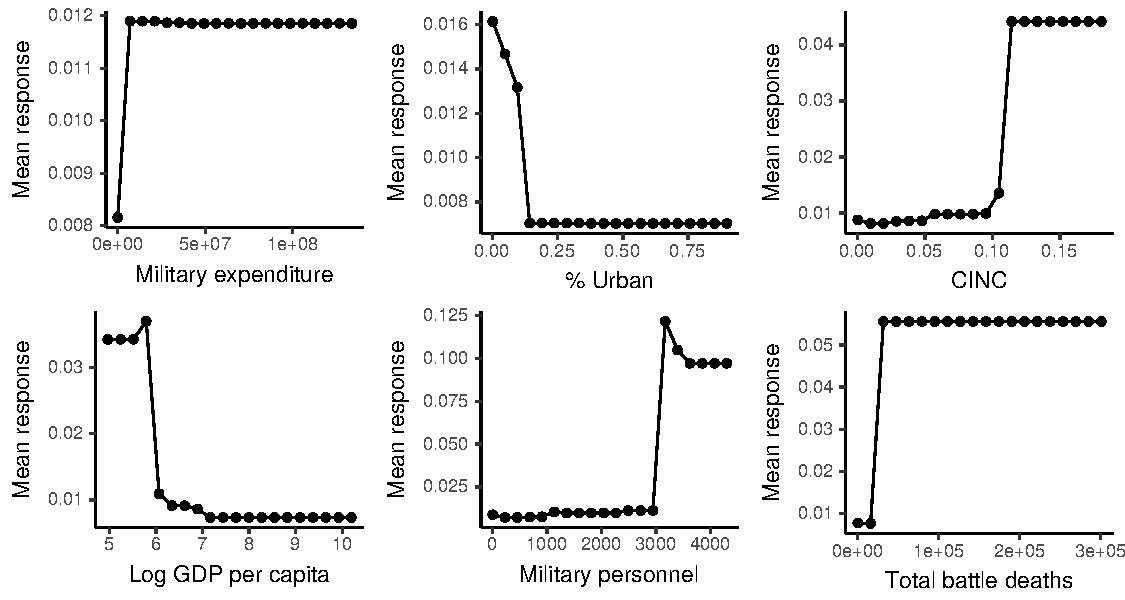
\includegraphics[width=\textwidth, height=9cm]{images/drfdpp7a.pdf}
    \caption{Partial Plots -- Genocides/Politicides (Cederman et al. Data)}
    \label{fig:my_label}
\end{figure}

\newpage

\subsection{\texttt{R} Code}
\label{sec:mk-code}

The \texttt{R} code below reproduces the analyses presented in the article.

\singlespacing
\footnotesize
\begin{verbatim}
######################
### Data Wrangling ###
######################

## Install and load required packages 
if (!require("tidyverse")) {
        install.packages("tidyverse")
}
if (!require("data.table")) {
        install.packages("data.table")
}
if (!require("ExtremeBounds")) {
        install.packages("ExtremeBounds")
}
if (!require("h2o")) {
        install.packages("h2o")
}
if (!require("sandwich")) {
        install.packages("sandwich")
}
if (!require("arm")) {
        install.packages("arm")
}
if (!require("stargazer")) {
        install.packages("stargazer")
}

## Load dataset
df <- haven::read_dta("data/base variables.dta") %>% setDT()

## Select and lag variables
sd.cols <- c("UCDPcivilwarstart", "UCDPcivilwarongoing", "COWcivilwarstart",
             "COWcivilwarongoing", "ethnowarstart", "ethnowarongoing",
             "assdummy", "demdummy", "elf", "lmtnest", "pop", "realgdp",
             "rgdppc", "polity2", "exclpop", "discpop", "polrqnew",
             "poltrqnew", "egiptpolrqnew", "egippolrqnew", "discrim",
             "elf2", "interstatewar", "milex", "milper", "percentpopurban",
             "postcoldwar", "coupdummy", "riotdummy", "territoryaims",
             "totaltrade", "tradedependence", "militias", "physint", "cinc",
             "totalbeaths", "change", "guerrilladummy", "sf", "regtrans")

df1 <- cbind(df, df[, shift(.SD, 1, give.names = TRUE),
                    by = ccode, .SDcols = sd.cols]) 

# Remove the second `ccode` variable
df1 <- as.data.frame(df1[, -c(70)])

# Add new variables
df1$logrgdppc_lag_1 <- log(df1$rgdppc_lag_1)
df1$polity2sq_lag_1 <- df1$polity2_lag_1^2

# UCDP civil war == 1
df.ucdp <- df1 %>% filter(UCDPcivilwarongoing == 1)
df.ucdp <- as.data.frame(df.ucdp[, c(1:7, 76:111)])
names(df.ucdp) <- sub("_.*","", names(df.ucdp)) 

# COW civil war == 1
df.cow <- df1 %>% filter(COWcivilwarongoing == 1)
df.cow <- as.data.frame(df.cow[, c(1:7, 76:111)])
names(df.cow) <- sub("_.*","", names(df.cow)) 

# Ethnic civil war == 1
df.eth <- df1 %>% filter(ethnowarongoing == 1)
df.eth <- as.data.frame(df.eth[, c(1:7, 76:111)])
names(df.eth) <- sub("_.*","", names(df.eth)) 

# Regular model
df2 <- as.data.frame(df1[, c(1:7, 70:111)])
names(df2) <- sub("_.*","", names(df2)) 


###############################
### Extreme Bounds Analyses ###
###############################

## Classifying a few variables as mutually exclusive.
## "Change" was removed because it was correlated at 0.99 with "regtrans". 
free.variables <- c("logrgdppc", "polity2", "mksyr")
civilwar.variables <- c("UCDPcivilwarongoing", "UCDPcivilwarstart",
                        "COWcivilwarongoing", "COWcivilwarstart",
                        "ethnowarongoing", "ethnowarstart")
doubtful.variables <- c("UCDPcivilwarongoing", "UCDPcivilwarstart",
                        "COWcivilwarongoing", "COWcivilwarstart",
                        "ethnowarongoing", "ethnowarstart", "assdummy",
                        "totaltrade", "tradedependence", "milper", "milex",
                        "pop", "totalbeaths", "guerrilladummy", "regtrans",
                        "riotdummy", "territoryaims", "militias",
                        "physint", "percentpopurban", "coupdummy",
                        "postcoldwar",  "lmtnest", "realgdp", "discrim",
                        "exclpop", "discpop", "elf",  "polrqnew",
                        "egippolrqnew", "poltrqnew", "egiptpolrqnew",
                        "polity2sq")

# Cluster-robust standard errors
se.clustered.robust <- function(model.object){
        model.fit <- vcovHC(model.object, type = "HC", cluster = "country")
        out <- sqrt(diag(model.fit))
        return(out)
}

# Main model
m1 <- eba(y = "MKstart", free = free.variables,
          exclusive = list(civilwar.variables),
          doubtful = doubtful.variables, k = 0:4,
          data = df2, vif = 7, level = 0.9,
          se.fun = se.clustered.robust)

summary(m1)
hist(m1, variables = c("logrgdppc", "polity2", "polity2sq", "mksyr",
                       "UCDPcivilwarongoing",
                       "UCDPcivilwarstart", "COWcivilwarongoing",
                       "COWcivilwarstart", "ethnowarongoing", "ethnowarstart",
                       "assdummy", "totaltrade", "tradedependence", "milper",
                       "milex","pop", "totalbeaths", "guerrilladummy", "regtrans",
                       "riotdummy", "territoryaims", "militias", "physint",
                       "percentpopurban", "coupdummy", "postcoldwar",
                       "lmtnest", "realgdp", "discrim", "exclpop", "discpop",
                       "elf", "polrqnew", "egippolrqnew", "poltrqnew",
                       "egiptpolrqnew"),
     main = c("Log GDP capita", "Polity IV", "Polity IV^2", "Years last mass killing",
              "UCDP ongoing", "UCDP onset", "COW ongoing", "COW onset", 
              "Ethnic ongoing", "Ethnic onset", "Assassination", "Total trade", 
              "Trade dependence", "Military personnel", "Military expenditure", "Population", 
              "Total deaths", "Guerrilla", "Regime transition", "Riots",
              "Territory Aims", "Militias", "Physical integrity", "% Urban",
              "Coups", "Post-Cold War", "Mountainous terrain", "Real GDP",
              "Discrimination", "Excl pop", "Discrim pop", "ELF", "Groups/Eth relevant", 
              "Group/Tot pop", "Inc groups/Eth relevant", "Inc groups/Tot pop"),
     density.col = "black", mu.col = "red3")
          
# Mass killings during civil war
# UCDP civil conflicts == 1
doubtful.variables <- c("assdummy", "totaltrade", "tradedependence",
                        "milper", "milex", "pop", "totalbeaths",
                        "guerrilladummy", "regtrans", "riotdummy",
                        "territoryaims", "militias", "physint",
                        "percentpopurban", "coupdummy", "postcoldwar",
                        "lmtnest", "realgdp", "discrim", "exclpop",
                        "discpop", "elf",  "polrqnew", "egippolrqnew",
                        "poltrqnew", "egiptpolrqnew", "polity2sq")

m1 <- eba(y = "MKstart", free = free.variables,
          doubtful = doubtful.variables, k = 0:4,
          data = df.ucdp, vif = 7,
          level = 0.9, se.fun = se.clustered.robust)
          
summary(m1)
hist(m1, variables = c("logrgdppc", "polity2", "polity2sq", "mksyr",
                       "assdummy", "totaltrade", "tradedependence", "milper",
                       "milex","pop", "totalbeaths", "guerrilladummy", "regtrans",
                       "riotdummy", "territoryaims", "militias", "physint",
                       "percentpopurban", "coupdummy", "postcoldwar",
                       "lmtnest", "realgdp", "discrim", "exclpop", "discpop",
                       "elf", "polrqnew", "egippolrqnew", "poltrqnew",
                       "egiptpolrqnew"),
     main = c("Log GDP capita", "Polity IV", "Polity IV^2", "Years last mass killing",
              "Assassination", "Total trade", 
              "Trade dependence", "Military personnel", "Military expenditure", "Population", 
              "Total deaths", "Guerrilla", "Regime transition", "Riots",
              "Territory Aims", "Militias", "Physical integrity", "% Urban",
              "Coups", "Post-Cold War", "Mountainous terrain", "Real GDP",
              "Discrimination", "Excl pop", "Discrim pop", "ELF", "Groups/Eth relevant", 
              "Group/Tot pop", "Inc groups/Eth relevant", "Inc groups/Tot pop"),
     density.col = "black", mu.col = "red3")
     
# COW civil wars == 1
doubtful.variables <- c("assdummy", "totaltrade", "tradedependence",
                        "milper", "milex", "pop", "totalbeaths",
                        "guerrilladummy", "regtrans", "riotdummy",
                        "territoryaims", "militias", "physint",
                        "percentpopurban", "coupdummy", "postcoldwar",
                        "lmtnest", "realgdp", "discrim", "exclpop",
                        "discpop", "elf",  "polrqnew", "egippolrqnew",
                        "poltrqnew", "egiptpolrqnew", "polity2sq")

m1 <- eba(y = "MKstart", free = free.variables,
          doubtful = doubtful.variables, k = 0:4,
          data = df.cow, vif = 7,
          level = 0.9, se.fun = se.clustered.robust)
          
summary(m1)
hist(m1, variables = c("logrgdppc", "polity2", "polity2sq", "mksyr",
                       "assdummy", "totaltrade", "tradedependence", "milper",
                       "milex","pop", "totalbeaths", "guerrilladummy", "regtrans",
                       "riotdummy", "territoryaims", "militias", "physint",
                       "percentpopurban", "coupdummy", "postcoldwar",
                       "lmtnest", "realgdp", "discrim", "exclpop", "discpop",
                       "elf", "polrqnew", "egippolrqnew", "poltrqnew",
                       "egiptpolrqnew"),
     main = c("Log GDP capita", "Polity IV", "Polity IV^2", "Years last mass killing",
              "Assassination", "Total trade", 
              "Trade dependence", "Military personnel", "Military expenditure", "Population", 
              "Total deaths", "Guerrilla", "Regime transition", "Riots",
              "Territory Aims", "Militias", "Physical integrity", "% Urban",
              "Coups", "Post-Cold War", "Mountainous terrain", "Real GDP",
              "Discrimination", "Excl pop", "Discrim pop", "ELF", "Groups/Eth relevant", 
              "Group/Tot pop", "Inc groups/Eth relevant", "Inc groups/Tot pop"),
     density.col = "black", mu.col = "red3")
     
# Ethnic civil war == 1
doubtful.variables <- c("assdummy", "totaltrade", "tradedependence",
                        "milper", "milex", "pop", "totalbeaths",
                        "guerrilladummy", "regtrans", "riotdummy",
                        "territoryaims", "militias", "physint",
                        "percentpopurban", "coupdummy", "postcoldwar",
                        "lmtnest", "realgdp", "discrim", "exclpop", 
                        "discpop", "elf",  "polrqnew", "egippolrqnew",
                        "poltrqnew", "egiptpolrqnew", "polity2sq")

m1 <- eba(y = "MKstart", free = free.variables,
          doubtful = doubtful.variables, k = 0:4,
          data = df.eth, vif = 7,
          level = 0.9, se.fun = se.clustered.robust)
          
summary(m1)
hist(m1, variables = c("logrgdppc", "polity2", "polity2sq", "mksyr",
                       "assdummy", "totaltrade", "tradedependence", "milper",
                       "milex","pop", "totalbeaths", "guerrilladummy", "regtrans",
                       "riotdummy", "territoryaims", "militias", "physint",
                       "percentpopurban", "coupdummy", "postcoldwar",
                       "lmtnest", "realgdp", "discrim", "exclpop", "discpop",
                       "elf", "polrqnew", "egippolrqnew", "poltrqnew",
                       "egiptpolrqnew"),
     main = c("Log GDP capita", "Polity IV", "Polity IV^2", "Years last mass killing",
              "Assassination", "Total trade", 
              "Trade dependence", "Military personnel", "Military expenditure", "Population", 
              "Total deaths", "Guerrilla", "Regime transition", "Riots",
              "Territory Aims", "Militias", "Physical integrity", "% Urban",
              "Coups", "Post-Cold War", "Mountainous terrain", "Real GDP",
              "Discrimination", "Excl pop", "Discrim pop", "ELF", "Groups/Eth relevant", 
              "Group/Tot pop", "Inc groups/Eth relevant", "Inc groups/Tot pop"),
     density.col = "black", mu.col = "red3")

## Different values of k
## Code for the histogram not included as it is the same as that of the main model.

# 3 variables per model
m1 <- eba(y = "MKstart", free = free.variables,
          exclusive = list(civilwar.variables),
          doubtful = doubtful.variables, k = 0:3,
          data = df2, vif = 7, level = 0.9, draws = 50000,
          se.fun = se.clustered.robust)

# 5 variables per model
m1 <- eba(y = "MKstart", free = free.variables,
          exclusive = list(civilwar.variables),
          doubtful = doubtful.variables, k = 0:5,
          data = df2, vif = 7, draws = 50000,
          level = 0.9, se.fun = se.clustered.robust)
          
## Alternative VIFs

# VIF = 10
# Low VIF
m1 <- eba(y = "MKstart", free = free.variables,
          exclusive = list(civilwar.variables),
          doubtful = doubtful.variables, k = 0:4,
          data = df2, vif = 10, level = 0.9, draws = 50000,
          se.fun = se.clustered.robust)

# VIF = 2.5
m1 <- eba(y = "MKstart", free = free.variables,
          exclusive = list(civilwar.variables),
          doubtful = doubtful.variables, k = 0:4,
          data = df2, vif = 2.5, level = 0.9, draws = 50000,
          se.fun = se.clustered.robust)

# No VIF
m1 <- eba(y = "MKstart", free = free.variables,
          exclusive = list(civilwar.variables),
          doubtful = doubtful.variables, k = 0:4,
          data = df2, level = 0.9, draws = 50000,
          se.fun = se.clustered.robust)

## Generalised linear models

# Logit
m1 <- eba(y = "MKstart", free = free.variables,
          exclusive = list(civilwar.variables),
          doubtful = doubtful.variables, k = 0:4,
          data = df2, level = 0.9, vif = 7, draws = 50000,
          reg.fun = bayesglm, family = binomial(link = "logit"))
          
# Probit
m1 <- eba(y = "MKstart", free = free.variables,
          exclusive = list(civilwar.variables),
          doubtful = doubtful.variables, k = 0:4,
          data = df2, level = 0.9, vif = 7, draws = 50000,
          reg.fun = bayesglm, family = binomial(link = "probit"))
          

##################################
### Distributed Random Forests ###
##################################

## Random Forests

## Prepare the data set
h2o.init(nthreads = -1, max_mem_size = "20g") # memory size

df2a <- as.h2o(df2)

df2a$MKstart <- as.factor(df2a$MKstart)  # encode the binary response as a factor
h2o.levels(df2a$MKstart)

# Partition the data into training, validation and test sets
splits <- h2o.splitFrame(data = df2a, 
                         ratios = c(0.7, 0.15),  # 70%, 15%, 15%
                         seed = 42)  # reproducibility

train <- h2o.assign(splits[[1]], "train.hex")   
valid <- h2o.assign(splits[[2]], "valid.hex") 
test <- h2o.assign(splits[[3]], "test.hex")

y <- "MKstart"
x <- setdiff(names(df2), c(y, "ccode", "year", "rgdppc",
                           "mksyr2", "mksyr3", "sf", "country",
                           "elf2", "polity2sq")) 

# Running the model
rf <- h2o.grid("randomForest", x = x, y = y, training_frame = train, 
               validation_frame = valid, nfolds = 5, grid_id = "gridrf01",
               fold_assignment = "Stratified",
               hyper_params = list(ntrees = c(256, 512, 1024),
                                   max_depth = c(10, 20, 40),
                                   mtries = c(5, 6, 7),
                                   balance_classes = c(TRUE, FALSE),
                                   sample_rate = c(0.5, 0.632, 0.95),
                                   col_sample_rate_per_tree = c(0.5, 0.9, 1.0),
                                   histogram_type = c("UniformAdaptive",
                                                      "Random",
                                                      "QuantilesGlobal",
                                                      "RoundRobin")),
               search_criteria = list(strategy = "RandomDiscrete", 
                                      max_models = 1000, 
                                      stopping_metric = "auc", 
                                      stopping_tolerance = 0.01, 
                                      stopping_rounds = 5, 
                                      seed = 26227709)) 

# Saving the most accurate model
rf.grid <- h2o.getGrid(grid_id = "gridrf01",
                       sort_by = "auc",
                       decreasing = TRUE)

rf2 <- h2o.getModel(rf.grid@model_ids[[1]])
h2o.saveModel(rf2, path = "/root/Documents/mk/")
summary(rf2)
varimp <- as.data.frame(h2o.varimp(rf2))
h2o.varimp_plot(rf2)
h2o.performance(rf2, newdata = test)

# Graphs
a <- h2o.loadModel("/home/sussa/Documents/GitHub/mk/gridrf01_model_21")
print(va <- a %>% h2o.varimp() %>% as.data.frame() %>% head(., 6)) 

par(mgp=c(2.2,0.45,0), tcl=-0.4, mar=c(2,7.5,1,1))
barplot(va$scaled_importance[6:1],
        horiz = TRUE, las = 1, cex.names=0.9,
        names.arg = c("Polity IV", 
                      "Military personnel",
                      "Ethnic polarisation", 
                      "% Urban pop.",
                      "Years mass killing",
                      "Log GDP per capita"),
        main = "")

logrgdppc <- h2o.partialPlot(object = a, data = train, cols = c("logrgdppc"))
p1 <- qplot(logrgdppc$logrgdppc, logrgdppc$mean_response) + geom_line() + theme_classic() + ylim(0, 0.05) +
        xlab("Log GDP per capita") + ylab("Mean response")

mksyr <- h2o.partialPlot(object = a, data = train, cols = c("mksyr"))
p2 <- qplot(mksyr$mksyr, mksyr$mean_response) + geom_line() + theme_classic() + ylim(0, 0.05) +
        xlab("Years since mass killing") +  ylab("Mean response")

percentpopurban <- h2o.partialPlot(object = a, data = train, cols = c("percentpopurban"))
p3 <- qplot(percentpopurban$percentpopurban, percentpopurban$mean_response) + geom_line() +
        theme_classic() + ylim(0, 0.05) + xlab("% Urban") + ylab("Mean response")

egiptpolrqnew <- h2o.partialPlot(object = a, data = train, cols = c("egiptpolrqnew"))
p4 <- qplot(egiptpolrqnew$egiptpolrqnew, egiptpolrqnew$mean_response) + geom_line() +
        theme_classic() + ylim(0, 0.05) + xlab("Ethnic polarisation") + ylab("Mean response")

milper <- h2o.partialPlot(object = a, data = train, cols = c("milper"))
p5 <- qplot(milper$milper, milper$mean_response) + geom_line() + theme_classic() + ylim(0, 0.05) +
        xlab("Military personnel") + ylab("Mean response")

polity2 <- h2o.partialPlot(object = a, data = train, cols = c("polity2"))
p6 <- qplot(polity2$polity2, polity2$mean_response) + geom_line() + theme_classic() + ylim(0, 0.05) +
        xlab("Polity IV") + ylab("Mean response")
        
# Multiplot function: http://www.cookbook-r.com/Graphs/Multiple_graphs_on_one_page_(ggplot2)/
multiplot <- function(..., plotlist=NULL, file, cols=1, layout=NULL) {
        library(grid)
        
        # Make a list from the ... arguments and plotlist
        plots <- c(list(...), plotlist)
        
        numPlots = length(plots)
        
        # If layout is NULL, then use 'cols' to determine layout
        if (is.null(layout)) {
                # Make the panel
                # ncol: Number of columns of plots
                # nrow: Number of rows needed, calculated from # of cols
                layout <- matrix(seq(1, cols * ceiling(numPlots/cols)),
                                 ncol = cols, nrow = ceiling(numPlots/cols))
        }
        
        if (numPlots==1) {
                print(plots[[1]])
                
        } else {
                # Set up the page
                grid.newpage()
                pushViewport(viewport(layout = grid.layout(nrow(layout), ncol(layout))))
                
                # Make each plot, in the correct location
                for (i in 1:numPlots) {
                        # Get the i,j matrix positions of the regions that contain this subplot
                        matchidx <- as.data.frame(which(layout == i, arr.ind = TRUE))
                        
                        print(plots[[i]], vp = viewport(layout.pos.row = matchidx$row,
                                                        layout.pos.col = matchidx$col))
                }
        }
}

multiplot(p1, p4, p2, p5, p3, p6, cols = 3)

## Different seeds

rf <- h2o.grid("randomForest", x = x, y = y, training_frame = train, 
               validation_frame = valid, nfolds = 5, grid_id = "gridrf01b",
               fold_assignment = "Stratified",
               hyper_params = list(ntrees = c(256, 512, 1024),
                                   max_depth = c(10, 20, 40),
                                   mtries = c(5, 6, 7),
                                   balance_classes = c(TRUE, FALSE),
                                   sample_rate = c(0.5, 0.632, 0.95),
                                   col_sample_rate_per_tree = c(0.5, 0.9, 1.0),
                                   histogram_type = c("UniformAdaptive",
                                                      "Random",
                                                      "QuantilesGlobal",
                                                      "RoundRobin")),
               search_criteria = list(strategy = "RandomDiscrete", 
                                      max_models = 1000, 
                                      stopping_metric = "auc", 
                                      stopping_tolerance = 0.01, 
                                      stopping_rounds = 5, 
                                      seed = 44849999)) 

# Saving the most accurate model
rf.grid <- h2o.getGrid(grid_id = "gridrf01b",
                       sort_by = "auc",
                       decreasing = TRUE)

rf2 <- h2o.getModel(rf.grid@model_ids[[1]])
h2o.saveModel(rf2, path = "/root/Documents/mk/")
summary(rf2)
varimp <- as.data.frame(h2o.varimp(rf2))
h2o.varimp_plot(rf2)
h2o.performance(rf2, newdata = test)

# Graphs
a <- h2o.loadModel("/home/sussa/Documents/GitHub/mk/gridrf01b_model_8")
print(va <- a %>% h2o.varimp() %>% as.data.frame() %>% head(., 6)) 

par(mgp=c(2.2,0.45,0), tcl=-0.4, mar=c(2,7.5,1,1))
barplot(va$scaled_importance[6:1],
        horiz = TRUE, las = 1, cex.names=0.9,
        names.arg = c("Population", 
                      "Military personnel",
                      "Trade dependence", 
                      "Log GDP per capita",
                      "% Urban pop.",
                      "Years mass killing"),
        main = "")

mksyr <- h2o.partialPlot(object = a, data = train, cols = c("mksyr"))
p1 <- qplot(mksyr$mksyr, mksyr$mean_response) + geom_line() + theme_classic() + ylim(0, 0.05) +
        xlab("Years since mass killing") +  ylab("Mean response")
        
percentpopurban <- h2o.partialPlot(object = a, data = train, cols = c("percentpopurban"))
p2 <- qplot(percentpopurban$percentpopurban, percentpopurban$mean_response) + geom_line() +
        theme_classic() + ylim(0, 0.05) + xlab("% Urban") + ylab("Mean response")

logrgdppc <- h2o.partialPlot(object = a, data = train, cols = c("logrgdppc"))
p3 <- qplot(logrgdppc$logrgdppc, logrgdppc$mean_response) + geom_line() + theme_classic() + ylim(0, 0.05) +
        xlab("Log GDP per capita") + ylab("Mean response")

tradedependence <- h2o.partialPlot(object = a, data = train, cols = c("tradedependence"))
p4 <- qplot(tradedependence$tradedependence, tradedependence$mean_response) + geom_line() +
        theme_classic() + ylim(0, 0.05) + xlab("Trade dependence") + ylab("Mean response")

milper <- h2o.partialPlot(object = a, data = train, cols = c("milper"))
p5 <- qplot(milper$milper, milper$mean_response) + geom_line() + theme_classic() + ylim(0, 0.05) +
        xlab("Military personnel") + ylab("Mean response")

pop <- h2o.partialPlot(object = a, data = train, cols = c("pop"))
p6 <- qplot(pop$pop, pop$mean_response) + geom_line() + theme_classic() + ylim(0, 0.05) +
        xlab("Population") + ylab("Mean response")

multiplot(p1, p4, p2, p5, p3, p6, cols = 3)


rf <- h2o.grid("randomForest", x = x, y = y, training_frame = train, 
               validation_frame = valid, nfolds = 5, grid_id = "gridrf01c",
               fold_assignment = "Stratified",
               hyper_params = list(ntrees = c(256, 512, 1024),
                                   max_depth = c(10, 20, 40),
                                   mtries = c(5, 6, 7),
                                   balance_classes = c(TRUE, FALSE),
                                   sample_rate = c(0.5, 0.632, 0.95),
                                   col_sample_rate_per_tree = c(0.5, 0.9, 1.0),
                                   histogram_type = c("UniformAdaptive",
                                                      "Random",
                                                      "QuantilesGlobal",
                                                      "RoundRobin")),
               search_criteria = list(strategy = "RandomDiscrete", 
                                      max_models = 1000, 
                                      stopping_metric = "auc", 
                                      stopping_tolerance = 0.01, 
                                      stopping_rounds = 5, 
                                      seed = 1502436)) 

# Saving the most accurate model
rf.grid <- h2o.getGrid(grid_id = "gridrf01c",
                       sort_by = "auc",
                       decreasing = TRUE)

rf2 <- h2o.getModel(rf.grid@model_ids[[1]])
h2o.saveModel(rf2, path = "/root/Documents/mk/")
summary(rf2)
varimp <- as.data.frame(h2o.varimp(rf2))
h2o.varimp_plot(rf2)
h2o.performance(rf2, newdata = test)

# Graphs
a <- h2o.loadModel("/home/sussa/Documents/GitHub/mk/gridrf01c_model_58")
print(va <- a %>% h2o.varimp() %>% as.data.frame() %>% head(., 6)) 

par(mgp=c(2.2,0.45,0), tcl=-0.4, mar=c(2,7.5,1,1))
barplot(va$scaled_importance[6:1],
        horiz = TRUE, las = 1, cex.names=0.9,
        names.arg = c("Population", 
                      "Military personnel",
                      "Trade dependence", 
                      "Log GDP per capita",
                      "% Urban pop.",
                      "Years mass killing"),
        main = "")

mksyr <- h2o.partialPlot(object = a, data = train, cols = c("mksyr"))
p1 <- qplot(mksyr$mksyr, mksyr$mean_response) + geom_line() + theme_classic() + ylim(0, 0.05) +
        xlab("Years since mass killing") +  ylab("Mean response")
        
percentpopurban <- h2o.partialPlot(object = a, data = train, cols = c("percentpopurban"))
p2 <- qplot(percentpopurban$percentpopurban, percentpopurban$mean_response) + geom_line() +
        theme_classic() + ylim(0, 0.05) + xlab("% Urban") + ylab("Mean response")

logrgdppc <- h2o.partialPlot(object = a, data = train, cols = c("logrgdppc"))
p3 <- qplot(logrgdppc$logrgdppc, logrgdppc$mean_response) + geom_line() + theme_classic() + ylim(0, 0.05) +
        xlab("Log GDP per capita") + ylab("Mean response")

tradedependence <- h2o.partialPlot(object = a, data = train, cols = c("tradedependence"))
p4 <- qplot(tradedependence$tradedependence, tradedependence$mean_response) + geom_line() +
        theme_classic() + ylim(0, 0.05) + xlab("Trade dependence") + ylab("Mean response")

milper <- h2o.partialPlot(object = a, data = train, cols = c("milper"))
p5 <- qplot(milper$milper, milper$mean_response) + geom_line() + theme_classic() + ylim(0, 0.05) +
        xlab("Military personnel") + ylab("Mean response")

pop <- h2o.partialPlot(object = a, data = train, cols = c("pop"))
p6 <- qplot(pop$pop, pop$mean_response) + geom_line() + theme_classic() + ylim(0, 0.05) +
        xlab("Population) + ylab("Mean response")

multiplot(p1, p4, p2, p5, p3, p6, cols = 3)

## Genocides in civil wars

## UCDP data
df.ucdpa <- as.h2o(df.ucdp)

df.ucdpa$MKstart <- as.factor(df.ucdpa$MKstart)  # encode the binary response as a factor
h2o.levels(df.ucdpa$MKstart)

# Partition the data into training, validation and test sets
splits <- h2o.splitFrame(data = df.ucdpa, 
                         ratios = c(0.7, 0.15),  # 70%, 15%, 15%
                         seed = 42)  # reproducibility

train <- h2o.assign(splits[[1]], "train.hex")   
valid <- h2o.assign(splits[[2]], "valid.hex") 
test <- h2o.assign(splits[[3]], "test.hex")

y <- "MKstart"
x <- setdiff(names(df.ucdp), c(y, "ccode", "year", "rgdppc",
                           "mksyr2", "mksyr3", "sf", "country",
                           "elf2", "polity2sq")) 

# Running the model
rf <- h2o.grid("randomForest", x = x, y = y, training_frame = train, 
               validation_frame = valid, nfolds = 5, grid_id = "gridrf02",
               fold_assignment = "Stratified",
               hyper_params = list(ntrees = c(256, 512, 1024),
                                   max_depth = c(10, 20, 40),
                                   mtries = c(5, 6, 7),
                                   balance_classes = c(TRUE, FALSE),
                                   sample_rate = c(0.5, 0.632, 0.95),
                                   col_sample_rate_per_tree = c(0.5, 0.9, 1.0),
                                   histogram_type = c("UniformAdaptive",
                                                      "Random",
                                                      "QuantilesGlobal",
                                                      "RoundRobin")),
               search_criteria = list(strategy = "RandomDiscrete", 
                                      max_models = 1000, 
                                      stopping_metric = "auc", 
                                      stopping_tolerance = 0.01, 
                                      stopping_rounds = 5, 
                                      seed = 26227709)) 

rf.grid <- h2o.getGrid(grid_id = "gridrf02",
                       sort_by = "auc",
                       decreasing = TRUE)
rf2 <- h2o.getModel(rf.grid@model_ids[[1]])
h2o.saveModel(rf2, path = "/root/Documents/mk/")
summary(rf2)
varimp <- as.data.frame(h2o.varimp(rf2))
h2o.varimp_plot(rf2)
h2o.performance(rf2, newdata = test)

# Graphs
a <- h2o.loadModel("/home/sussa/Documents/GitHub/mk/gridrf02_model_34")
print(va <- a %>% h2o.varimp() %>% as.data.frame() %>% head(., 6)) 

par(mgp=c(2.2,0.45,0), tcl=-0.4, mar=c(2,7.5,1,1))
barplot(va$scaled_importance[6:1],
        horiz = TRUE, las = 1, cex.names=0.9,
        names.arg = c("Total battle deaths", 
                      "Log GDP per capita",
                       "Trade dependence",
                      "Military personnel",
                      "% Urban pop.",
                      "Years mass killing"),
        main = "")
        
mksyr <- h2o.partialPlot(object = a, data = train, cols = c("mksyr"))
p1 <- qplot(mksyr$mksyr, mksyr$mean_response) + geom_line() + theme_classic() + 
        ylim(0, 0.1) + xlab("Years since mass killing") +  ylab("Mean response")

percentpopurban <- h2o.partialPlot(object = a, data = train, cols = c("percentpopurban"))
p2 <- qplot(percentpopurban$percentpopurban, percentpopurban$mean_response) + geom_line() +
        ylim(0, 0.1) + theme_classic() + xlab("% Urban") + ylab("Mean response")

milper <- h2o.partialPlot(object = a, data = train, cols = c("milper"))
p3 <- qplot(milper$milper, milper$mean_response) + geom_line() + theme_classic() +
        ylim(0, 0.25) + xlab("Military personnel") + ylab("Mean response")

tradedependence <- h2o.partialPlot(object = a, data = train, cols = c("tradedependence"))
p4 <- qplot(tradedependence$tradedependence, tradedependence$mean_response) + geom_line() + theme_classic() +
        ylim(0, 0.1) + xlab("Trade dependence") + ylab("Mean response")

logrgdppc <- h2o.partialPlot(object = a, data = train, cols = c("logrgdppc"))
p5 <- qplot(logrgdppc$logrgdppc, logrgdppc$mean_response) + geom_line() + theme_classic() +
        ylim(0, 0.1) + xlab("Log GDP per capita") + ylab("Mean response")

totalbeaths <- h2o.partialPlot(object = a, data = train, cols = c("totalbeaths"))
p6 <- qplot(totalbeaths$totalbeaths, totalbeaths$mean_response) + geom_line() + theme_classic() +
        ylim(0, 0.35) + xlab("Total battle deaths") + ylab("Mean response")

multiplot(p1, p4, p2, p5, p3, p6, cols = 3)

## COW data
df.cowa <- as.h2o(df.cow)

df.cowa$MKstart <- as.factor(df.cowa$MKstart)
h2o.levels(df.cowa$MKstart)

# Partition the data into training, validation and test sets
splits <- h2o.splitFrame(data = df.cowa, 
                         ratios = c(0.7, 0.15),  # 70%, 15%, 15%
                         seed = 42) 

train <- h2o.assign(splits[[1]], "train.hex")   
valid <- h2o.assign(splits[[2]], "valid.hex") 
test <- h2o.assign(splits[[3]], "test.hex")

y <- "MKstart"
x <- setdiff(names(df.ucdp), c(y, "ccode", "year", "rgdppc",
                               "mksyr2", "mksyr3", "sf", "country",
                               "elf2", "polity2sq")) 

# Running the model
rf <- h2o.grid("randomForest", x = x, y = y, training_frame = train, 
               validation_frame = valid, nfolds = 5, grid_id = "gridrf03",
               fold_assignment = "Stratified",
               hyper_params = list(ntrees = c(256, 512, 1024),
                                   max_depth = c(10, 20, 40),
                                   mtries = c(5, 6, 7),
                                   balance_classes = c(TRUE, FALSE),
                                   sample_rate = c(0.5, 0.632, 0.95),
                                   col_sample_rate_per_tree = c(0.5, 0.9, 1.0),
                                   histogram_type = c("UniformAdaptive",
                                                      "Random",
                                                      "QuantilesGlobal",
                                                      "RoundRobin")),
               search_criteria = list(strategy = "RandomDiscrete", 
                                      max_models = 1000, 
                                      stopping_metric = "auc", 
                                      stopping_tolerance = 0.01, 
                                      stopping_rounds = 5, 
                                      seed = 26227709)) 

rf.grid <- h2o.getGrid(grid_id = "gridrf03",
                       sort_by = "auc",
                       decreasing = TRUE)
rf2 <- h2o.getModel(rf.grid@model_ids[[1]])
h2o.saveModel(rf2, path = "/root/Documents/mk/")
summary(rf2)
varimp <- as.data.frame(h2o.varimp(rf2))
h2o.varimp_plot(rf2)
h2o.performance(rf2, newdata = test)

## Graphs
a <- h2o.loadModel("/root/Documents/mk/gridrf03_model_3")
print(va <- a %>% h2o.varimp() %>% as.data.frame() %>% head(., 6)) 
par(mgp=c(2.2,0.45,0), tcl=-0.4, mar=c(2,7.5,1,1))
barplot(va$scaled_importance[6:1],
        horiz = TRUE, las = 1, cex.names=0.9,
        names.arg = c("Total battle deaths", 
                      "Excluded population",
                      "Yrs since mass killing",
                      "Log GDP per capita",
                      "Ethnic polarisation",
                      "Physical integrity"),
        main = "")

physint <- h2o.partialPlot(object = a, data = train, cols = c("physint"))
p1 <- qplot(physint$physint, physint$mean_response) + geom_line() + theme_classic() + 
        xlab("Physical integrity") +  ylab("Mean response")

egiptpolrqnew <- h2o.partialPlot(object = a, data = train, cols = c("egiptpolrqnew"))
p2 <- qplot(egiptpolrqnew$egiptpolrqnew, egiptpolrqnew$mean_response) + geom_line() +
        theme_classic() + xlab("Ethnic polarisation") + ylab("Mean response")

logrgdppc <- h2o.partialPlot(object = a, data = train, cols = c("logrgdppc"))
p3 <- qplot(logrgdppc$logrgdppc, logrgdppc$mean_response) + geom_line() + theme_classic() +
        ylim(0, 0.1) + xlab("Log GDP per capita") + ylab("Mean response")

mksyr <- h2o.partialPlot(object = a, data = train, cols = c("mksyr"))
p4 <- qplot(mksyr$mksyr, mksyr$mean_response) + geom_line() + theme_classic() + 
        ylim(0, 0.1) + xlab("Years since mass killing") +  ylab("Mean response")

exclpop <- h2o.partialPlot(object = a, data = train, cols = c("exclpop"))
p5 <- qplot(exclpop$exclpop, exclpop$mean_response) + geom_line() + theme_classic() +
        ylim(0, 0.1) + xlab("Excluded population") + ylab("Mean response")

totalbeaths <- h2o.partialPlot(object = a, data = train, cols = c("totalbeaths"))
p6 <- qplot(totalbeaths$totalbeaths, totalbeaths$mean_response) + geom_line() + theme_classic() +
        ylim(0, 0.1) + xlab("Total battle deaths") + ylab("Mean response")

multiplot(p1, p4, p2, p5, p3, p6, cols = 3)

## Ethnic war
df.etha <- as.h2o(df.eth)

df.etha$MKstart <- as.factor(df.etha$MKstart) 
h2o.levels(df.etha$MKstart)

# Partition the data into training, validation and test sets
splits <- h2o.splitFrame(data = df.etha, 
                         ratios = c(0.7, 0.15), 
                         seed = 42) 

train <- h2o.assign(splits[[1]], "train.hex")   
valid <- h2o.assign(splits[[2]], "valid.hex") 
test <- h2o.assign(splits[[3]], "test.hex")

y <- "MKstart"
x <- setdiff(names(df.eth), c(y, "ccode", "year", "rgdppc",
                               "mksyr2", "mksyr3", "sf", "country",
                               "elf2", "polity2sq")) 

# Running the model
rf <- h2o.grid("randomForest", x = x, y = y, training_frame = train, 
               validation_frame = valid, nfolds = 5, grid_id = "gridrf04",
               fold_assignment = "Stratified",
               hyper_params = list(ntrees = c(256, 512, 1024),
                                   max_depth = c(10, 20, 40),
                                   mtries = c(5, 6, 7),
                                   balance_classes = c(TRUE, FALSE),
                                   sample_rate = c(0.5, 0.632, 0.95),
                                   col_sample_rate_per_tree = c(0.5, 0.9, 1.0),
                                   histogram_type = c("UniformAdaptive",
                                                      "Random",
                                                      "QuantilesGlobal",
                                                      "RoundRobin")),
               search_criteria = list(strategy = "RandomDiscrete", 
                                      max_models = 1000, 
                                      stopping_metric = "auc", 
                                      stopping_tolerance = 0.01, 
                                      stopping_rounds = 5, 
                                      seed = 26227709)) 

rf.grid <- h2o.getGrid(grid_id = "gridrf04",
                       sort_by = "auc",
                       decreasing = TRUE)
rf2 <- h2o.getModel(rf.grid@model_ids[[1]])
h2o.saveModel(rf2, path = "/root/Documents/mk/")
summary(rf2)
varimp <- as.data.frame(h2o.varimp(rf2))
h2o.varimp_plot(rf2)
h2o.performance(rf2, newdata = test)

# Graphs
a <- h2o.loadModel("/root/Documents/mk/gridrf04_model_14")
print(va <- a %>% h2o.varimp() %>% as.data.frame() %>% head(., 6)) 

par(mgp=c(2.2,0.45,0), tcl=-0.4, mar=c(2,7.5,1,1))
barplot(va$scaled_importance[6:1],
        horiz = TRUE, las = 1, cex.names=0.9,
        names.arg = c("Military expenditure",
                      "Total trade", 
                      "% Urban",
                      "Trade dependence",
                      "Military personnel",
                      "CINC"),
        main = "")


cinc <- h2o.partialPlot(object = a, data = train, cols = c("cinc"))
p1 <- qplot(cinc$cinc, cinc$mean_response) + geom_line() + theme_classic() + 
        xlab("CINC") +  ylab("Mean response")

milper <- h2o.partialPlot(object = a, data = train, cols = c("milper"))
p2 <- qplot(milper$milper, milper$mean_response) + geom_line() +
        theme_classic() + xlab("Military personnel") + ylab("Mean response")

tradedependence <- h2o.partialPlot(object = a, data = train, cols = c("tradedependence"))
p3 <- qplot(tradedependence$tradedependence, tradedependence$mean_response) + geom_line() + theme_classic() +
        xlab("Trade dependence") + ylab("Mean response")

percentpopurban <- h2o.partialPlot(object = a, data = train, cols = c("percentpopurban"))
p4 <- qplot(percentpopurban$percentpopurban, percentpopurban$mean_response) + geom_line() +
       theme_classic() + xlab("% Urban") + ylab("Mean response")

totaltrade <- h2o.partialPlot(object = a, data = train, cols = c("totaltrade"))
p5 <- qplot(totaltrade$totaltrade, totaltrade$mean_response) + geom_line() +
        theme_classic() + xlab("Total trade") + ylab("Mean response")

milex <- h2o.partialPlot(object = a, data = train, cols = c("milex"))
p6 <- qplot(milex$milex, milex$mean_response) + geom_line() +
        theme_classic() + xlab("Military expenditure") + ylab("Mean response")

multiplot(p1, p4, p2, p5, p3, p6, cols = 3)

####################################
### Genocide/Politicide Variable ###
####################################

## The code below replicates the same analyses presented above
## but using a measure of genocide/politicide coded by Harff (2003).

## Data wrangling
df3 <- haven::read_dta("data/uamkstart.dta") %>% setDT()

sd.cols <- c("UCDPcivilwarstart", "UCDPcivilwarongoing", "COWcivilwarstart",
             "COWcivilwarongoing", "ethnowarstart", "ethnowarongoing",
             "assdummy", "demdummy", "elf", "lmtnest", "pop", "realgdp",
             "rgdppc", "polity2", "exclpop", "discpop", "polrqnew",
             "poltrqnew", "egiptpolrqnew", "egippolrqnew", "discrim",
             "elf2", "interstatewar", "milex", "milper", "percentpopurban",
             "postcoldwar", "coupdummy", "riotdummy", "territoryaims",
             "totaltrade", "tradedependence", "militias", "physint", "cinc",
             "totalbeaths", "change", "guerrilladummy", "sf", "regtrans")

df4 <- cbind(df3, df3[, shift(.SD, 1, give.names = TRUE),
                      by = ccode, .SDcols = sd.cols]) 

# Remove the second `ccode` variable
df4 <- as.data.frame(df4[, -c(75)])

# Add new variables
df4$logrgdppc_lag_1 <- log(df4$rgdppc_lag_1)
df4$polity2sq_lag_1 <- df4$polity2_lag_1^2

# Renaming variables
df5 <- as.data.frame(df4[, c(1:4, 72:116)])
names(df5) <- sub("_.*","", names(df5)) 

#################################################
### Distributed Random Forests - Harff (2003) ###
#################################################

df5a <- as.h2o(df5)

df5a$uamkstart <- as.factor(df5a$uamkstart)  #encode the binary repsonse as a factor
h2o.levels(df5a$uamkstart)

# Partition the data into training, validation and test sets
splits <- h2o.splitFrame(data = df5a, 
                         ratios = c(0.7, 0.15),  # 70%, 15%, 15%
                         seed = 42)  # reproducibility


train <- h2o.assign(splits[[1]], "train.hex")   
valid <- h2o.assign(splits[[2]], "valid.hex") 
test <- h2o.assign(splits[[3]], "test.hex")

y <- "uamkstart"
x <- setdiff(names(df5), c(y, "ccode", "year", "rgdppc",
                           "uamkyr2", "uamkyr3", "sf", "country",
                           "elf2", "polity2sq")) 
# Running the model
rf <- h2o.grid("randomForest", x = x, y = y, training_frame = train, 
               validation_frame = valid, nfolds = 5, 
               grid_id = "gridrf05",
               fold_assignment = "Stratified",
               hyper_params = list(ntrees = c(256, 512, 1024),
                                   max_depth = c(10, 20, 40),
                                   mtries = c(5, 6, 7),
                                   balance_classes = c(TRUE, FALSE),
                                   sample_rate = c(0.5, 0.632, 0.95),
                                   col_sample_rate_per_tree = c(0.5, 0.9, 1.0),
                                   histogram_type = c("UniformAdaptive",
                                                      "Random",
                                                      "QuantilesGlobal",
                                                      "RoundRobin")),
               search_criteria = list(strategy = "RandomDiscrete", 
                                      max_models = 1000, 
                                      stopping_metric = "auc", 
                                      stopping_tolerance = 0.01, 
                                      stopping_rounds = 5, 
                                      seed = 26227709)) 
                                      
# Saving the most accurate model
rf.grid <- h2o.getGrid(grid_id = "gridrf05",
                       sort_by = "auc",
                       decreasing = TRUE)

rf2 <- h2o.getModel(rf.grid@model_ids[[1]])
h2o.saveModel(rf2, path = "/root/Documents/mk/")
summary(rf2)
varimp <- as.data.frame(h2o.varimp(rf2))
h2o.varimp_plot(rf2)
h2o.performance(rf2, newdata = test)

## Graphs
a <- h2o.loadModel("/home/sussa/Documents/GitHub/mk/gridrf05_model_27")
print(va <- a %>% h2o.varimp() %>% as.data.frame() %>% head(., 6)) 

par(mgp=c(2.2,0.45,0), tcl=-0.4, mar=c(2,7.5,1,1))
barplot(va$scaled_importance[6:1],
        horiz = TRUE, las = 1, cex.names=0.9,
        names.arg = c("Real GDP", 
                      "Military expenditure",
                      "Total trade", 
                      "Military personnel",
                      "CINC", 
                      "% Urban"),
        main = "")

percentpopurban <- h2o.partialPlot(object = a, data = train, cols = c("percentpopurban"))
p1 <- qplot(percentpopurban$percentpopurban, percentpopurban$mean_response) + geom_line() +
        theme_classic() + xlab("% Urban") + ylab("Mean response")
        
cinc <- h2o.partialPlot(object = a, data = train, cols = c("cinc"))
p2 <- qplot(cinc$cinc, cinc$mean_response) + geom_line() + theme_classic() + 
        xlab("CINC") +  ylab("Mean response")

milper <- h2o.partialPlot(object = a, data = train, cols = c("milper"))
p3 <- qplot(milper$milper, milper$mean_response) + geom_line() +
        theme_classic() + xlab("Military personnel") + ylab("Mean response")

totaltrade <- h2o.partialPlot(object = a, data = train, cols = c("totaltrade"))
p4 <- qplot(totaltrade$totaltrade, totaltrade$mean_response) + geom_line() + theme_classic() +
        xlab("Total trade") + ylab("Mean response")

milex <- h2o.partialPlot(object = a, data = train, cols = c("milex"))
p5 <- qplot(milex$milex, milex$mean_response) + geom_line() +
        theme_classic() + xlab("Military expenditure") + ylab("Mean response")
        
realgdp <- h2o.partialPlot(object = a, data = train, cols = c("realgdp"))
p6 <- qplot(realgdp$realgdp, realgdp$mean_response) + geom_line() +
        theme_classic() + xlab("Real GDP") + ylab("Mean response")

multiplot(p1, p4, p2, p5, p3, p6, cols = 3)


## UCDP == 1
df.ucdp2 <- df5 %>% filter(UCDPcivilwarongoing == 1)
df.ucdp2a <- as.h2o(df.ucdp2)

df.ucdp2a$uamkstart <- as.factor(df.ucdp2a$uamkstart)  #encode the binary repsonse as a factor
h2o.levels(df.ucdp2a$uamkstart)

# Partition the data into training, validation and test sets
splits <- h2o.splitFrame(data = df.ucdp2a, 
                         ratios = c(0.7, 0.15),  # 70%, 15%, 15%
                         seed = 42)  # reproducibility


train <- h2o.assign(splits[[1]], "train.hex")   
valid <- h2o.assign(splits[[2]], "valid.hex") 
test <- h2o.assign(splits[[3]], "test.hex")

y <- "uamkstart"
x <- setdiff(names(df.ucdp2), c(y, "ccode", "year", "rgdppc",
                           "uamkyr2", "uamkyr3", "sf", "country",
                           "elf2", "polity2sq")) 

# Running the model
rf <- h2o.grid("randomForest", x = x, y = y, training_frame = train, 
               validation_frame = valid, nfolds = 5, grid_id = "gridrf06",
               fold_assignment = "Stratified",
               hyper_params = list(ntrees = c(256, 512, 1024),
                                   max_depth = c(10, 20, 40),
                                   mtries = c(5, 6, 7),
                                   balance_classes = c(TRUE, FALSE),
                                   sample_rate = c(0.5, 0.632, 0.95),
                                   col_sample_rate_per_tree = c(0.5, 0.9, 1.0),
                                   histogram_type = c("UniformAdaptive",
                                                      "Random",
                                                      "QuantilesGlobal",
                                                      "RoundRobin")),
               search_criteria = list(strategy = "RandomDiscrete", 
                                      max_models = 1000, 
                                      stopping_metric = "auc", 
                                      stopping_tolerance = 0.01, 
                                      stopping_rounds = 5, 
                                      seed = 26227709)) 

rf.grid <- h2o.getGrid(grid_id = "gridrf06",
                       sort_by = "auc",
                       decreasing = TRUE)
rf2 <- h2o.getModel(rf.grid@model_ids[[1]])
h2o.saveModel(rf2, path = "/root/Documents/mk/")
summary(rf2)
varimp <- as.data.frame(h2o.varimp(rf2))
h2o.varimp_plot(rf2)
h2o.performance(rf2, newdata = test)

## Graphs
a <- h2o.loadModel("/home/sussa/Documents/GitHub/mk/gridrf06_model_43")
print(va <- a %>% h2o.varimp() %>% as.data.frame() %>% head(., 6)) 

par(mgp=c(2.2,0.45,0), tcl=-0.4, mar=c(2,7.5,1,1))
barplot(va$scaled_importance[6:1],
        horiz = TRUE, las = 1, cex.names=0.9,
        names.arg = c("Excluded population",
                      "% Urban pop.", 
                      "Trade dependence",
                      "Log GDP per capita",
                      "Years since genocide", 
                      "Military personnel"),
        main = "")
        
milper <- h2o.partialPlot(object = a, data = train, cols = c("milper"))
p1 <- qplot(milper$milper, milper$mean_response) + geom_line() +
        theme_classic() + xlab("Military personnel") + ylab("Mean response")

uamkyr <- h2o.partialPlot(object = a, data = train, cols = c("uamkyr"))
p2 <- qplot(uamkyr$uamkyr, uamkyr$mean_response) + geom_line() + theme_classic() + 
        xlab("Years since genocide") +  ylab("Mean response")
        
logrgdppc <- h2o.partialPlot(object = a, data = train, cols = c("logrgdppc"))
p3 <- qplot(logrgdppc$logrgdppc, logrgdppc$mean_response) + geom_line() + theme_classic() +
        xlab("Log GDP per capita") + ylab("Mean response")

tradedependence <- h2o.partialPlot(object = a, data = train, cols = c("tradedependence"))
p4 <- qplot(tradedependence$tradedependence, tradedependence$mean_response) + geom_line() +
        theme_classic() + xlab("Trade dependence") + ylab("Mean response")

percentpopurban <- h2o.partialPlot(object = a, data = train, cols = c("percentpopurban"))
p5 <- qplot(percentpopurban$percentpopurban, percentpopurban$mean_response) + geom_line() +
        theme_classic() + xlab("% Urban") + ylab("Mean response")
        
exclpop <- h2o.partialPlot(object = a, data = train, cols = c("exclpop"))
p6 <- qplot(exclpop$exclpop, exclpop$mean_response) + geom_line() +
        theme_classic() + xlab("Excluded population") + ylab("Mean response")

multiplot(p1, p4, p2, p5, p3, p6, cols = 3)

## COW == 1
df.cow2 <- df5 %>% filter(COWcivilwarongoing == 1)

df.cow2a$uamkstart <- as.factor(df.cow2a$uamkstart)  #encode the binary repsonse as a factor
h2o.levels(df.cow2a$uamkstart)

# Partition the data into training, validation and test sets
splits <- h2o.splitFrame(data = df.cow2a, 
                         ratios = c(0.7, 0.15),  # 70%, 15%, 15%
                         seed = 42)  # reproducibility


train <- h2o.assign(splits[[1]], "train.hex")   
valid <- h2o.assign(splits[[2]], "valid.hex") 
test <- h2o.assign(splits[[3]], "test.hex")

y <- "uamkstart"
x <- setdiff(names(df.cow2), c(y, "ccode", "year", "rgdppc",
                               "uamkyr2", "uamkyr3", "sf", "country",
                               "elf2", "polity2sq")) 

## Running the model
rf <- h2o.grid("randomForest", x = x, y = y, training_frame = train, 
               validation_frame = valid, nfolds = 5, grid_id = "gridrf07",
               fold_assignment = "Stratified",
               hyper_params = list(ntrees = c(256, 512, 1024),
                                   max_depth = c(10, 20, 40),
                                   mtries = c(5, 6, 7),
                                   balance_classes = c(TRUE, FALSE),
                                   sample_rate = c(0.5, 0.632, 0.95),
                                   col_sample_rate_per_tree = c(0.5, 0.9, 1.0),
                                   histogram_type = c("UniformAdaptive",
                                                      "Random",
                                                      "QuantilesGlobal",
                                                      "RoundRobin")),
               search_criteria = list(strategy = "RandomDiscrete", 
                                      max_models = 1000, 
                                      stopping_metric = "auc", 
                                      stopping_tolerance = 0.01, 
                                      stopping_rounds = 5, 
                                      seed = 26227709)) 

rf.grid <- h2o.getGrid(grid_id = "gridrf07",
                       sort_by = "auc",
                       decreasing = TRUE)
rf2 <- h2o.getModel(rf.grid@model_ids[[1]])
h2o.saveModel(rf2, path = "/root/Documents/mk/")
summary(rf2)
varimp <- as.data.frame(h2o.varimp(rf2))
h2o.varimp_plot(rf2)
h2o.performance(rf2, newdata = test)

## Graphs
a <- h2o.loadModel("/home/sussa/Documents/GitHub/mk/gridrf07_model_27")
print(va <- a %>% h2o.varimp() %>% as.data.frame() %>% head(., 6)) 

par(mgp=c(2.2,0.45,0), tcl=-0.4, mar=c(2,7.5,1,1))
barplot(va$scaled_importance[6:1],
        horiz = TRUE, las = 1, cex.names=0.9,
        names.arg = c("Military expenditure",
                      "% Urban pop.", 
                      "Total trade",
                      "Years since genocide", 
                      "Military personnel", 
                      "Trade dependence"),
        main = "")

uamkyr <- h2o.partialPlot(object = a, data = train, cols = c("uamkyr"))
p3 <- qplot(uamkyr$uamkyr, uamkyr$mean_response) + geom_line() + theme_classic() + 
        xlab("Years since genocide") +  ylab("Mean response")

milper <- h2o.partialPlot(object = a, data = train, cols = c("milper"))
p2 <- qplot(milper$milper, milper$mean_response) + geom_line() +
        theme_classic() + xlab("Military personnel") + ylab("Mean response")

totaltrade <- h2o.partialPlot(object = a, data = train, cols = c("totaltrade"))
p4 <- qplot(totaltrade$totaltrade, totaltrade$mean_response) + geom_line() + theme_classic() +
        xlab("Total trade") + ylab("Mean response")

percentpopurban <- h2o.partialPlot(object = a, data = train, cols = c("percentpopurban"))
p5 <- qplot(percentpopurban$percentpopurban, percentpopurban$mean_response) + geom_line() +
        theme_classic() + xlab("% Urban") + ylab("Mean response")

tradedependence <- h2o.partialPlot(object = a, data = train, cols = c("tradedependence"))
p1 <- qplot(tradedependence$tradedependence, tradedependence$mean_response) + geom_line() +
        theme_classic() + xlab("Trade dependence") + ylab("Mean response")

milex <- h2o.partialPlot(object = a, data = train, cols = c("milex"))
p6 <- qplot(milex$milex, milex$mean_response) + geom_line() +
        theme_classic() + xlab("Military expenditure") + ylab("Mean response")

multiplot(p1, p4, p2, p5, p3, p6, cols = 3)

## ETHONSET == 1
df.eth2 <- df5 %>% filter(ethnowarongoing == 1)

df.eth2a <- as.h2o(df.eth2)

df.eth2a$uamkstart <- as.factor(df.eth2a$uamkstart)  #encode the binary repsonse as a factor
h2o.levels(df.eth2a$uamkstart)

# Partition the data into training, validation and test sets
splits <- h2o.splitFrame(data = df.eth2a, 
                         ratios = c(0.7, 0.15),  # 70%, 15%, 15%
                         seed = 42)  # reproducibility


train <- h2o.assign(splits[[1]], "train.hex")   
valid <- h2o.assign(splits[[2]], "valid.hex") 
test <- h2o.assign(splits[[3]], "test.hex")

y <- "uamkstart"
x <- setdiff(names(df.eth2), c(y, "ccode", "year", "rgdppc",
                               "uamkyr2", "uamkyr3", "sf", "country",
                               "elf2", "polity2sq")) 

# Running the model
rf <- h2o.grid("randomForest", x = x, y = y, training_frame = train, 
               validation_frame = valid, nfolds = 5, grid_id = "gridrf08",
               fold_assignment = "Stratified",
               hyper_params = list(ntrees = c(256, 512, 1024),
                                   max_depth = c(10, 20, 40),
                                   mtries = c(5, 6, 7),
                                   balance_classes = c(TRUE, FALSE),
                                   sample_rate = c(0.5, 0.632, 0.95),
                                   col_sample_rate_per_tree = c(0.5, 0.9, 1.0),
                                   histogram_type = c("UniformAdaptive",
                                                      "Random",
                                                      "QuantilesGlobal",
                                                      "RoundRobin")),
               search_criteria = list(strategy = "RandomDiscrete", 
                                      max_models = 1000, 
                                      stopping_metric = "auc", 
                                      stopping_tolerance = 0.01, 
                                      stopping_rounds = 5, 
                                      seed = 26227709)) 

rf.grid <- h2o.getGrid(grid_id = "gridrf08",
                       sort_by = "auc",
                       decreasing = TRUE)
rf2 <- h2o.getModel(rf.grid@model_ids[[1]])
h2o.saveModel(rf2, path = "/root/Documents/mk/")
summary(rf2)
varimp <- as.data.frame(h2o.varimp(rf2))
h2o.varimp_plot(rf2)
h2o.performance(rf2, newdata = test)

## Graphs
a <- h2o.loadModel("/home/sussa/Documents/GitHub/mk/gridrf08_model_55")
print(va <- a %>% h2o.varimp() %>% as.data.frame() %>% head(., 6)) 

par(mgp=c(2.2,0.45,0), tcl=-0.4, mar=c(2,7.5,1,1))
barplot(va$scaled_importance[6:1],
        horiz = TRUE, las = 1, cex.names=0.9,
        names.arg = c("Total battle deaths", 
                      "Military personnel",
                      "Log GDP per capita", 
                      "CINC",
                      "% Urban",
                      "Military expenditure"),
        main = "")

cinc <- h2o.partialPlot(object = a, data = train, cols = c("cinc"))
p3 <- qplot(cinc$cinc, cinc$mean_response) + geom_line() + theme_classic() + 
        xlab("CINC") +  ylab("Mean response")

milper <- h2o.partialPlot(object = a, data = train, cols = c("milper"))
p5 <- qplot(milper$milper, milper$mean_response) + geom_line() +
        theme_classic() + xlab("Military personnel") + ylab("Mean response")

logrgdppc <- h2o.partialPlot(object = a, data = train, cols = c("logrgdppc"))
p4 <- qplot(logrgdppc$logrgdppc, logrgdppc$mean_response) + geom_line() + theme_classic() +
        xlab("Log GDP per capita") + ylab("Mean response")

percentpopurban <- h2o.partialPlot(object = a, data = train, cols = c("percentpopurban"))
p2 <- qplot(percentpopurban$percentpopurban, percentpopurban$mean_response) + geom_line() +
        theme_classic() + xlab("% Urban") + ylab("Mean response")

totalbeaths <- h2o.partialPlot(object = a, data = train, cols = c("totalbeaths"))
p6 <- qplot(totalbeaths$totalbeaths, totalbeaths$mean_response) + geom_line() +
        theme_classic() + xlab("Total battle deaths") + ylab("Mean response")

milex <- h2o.partialPlot(object = a, data = train, cols = c("milex"))
p1 <- qplot(milex$milex, milex$mean_response) + geom_line() +
        theme_classic() + xlab("Military expenditure") + ylab("Mean response")

multiplot(p1, p4, p2, p5, p3, p6, cols = 3)


##############################################
### Genocides and Politicides (Harff 2003) ###
##############################################

# Preparing the dataset
df3 <- haven::read_dta("data/uamkstart.dta") %>% setDT()
sd.cols <- c("UCDPcivilwarstart", "UCDPcivilwarongoing", "COWcivilwarstart",
             "COWcivilwarongoing", "ethnowarstart", "ethnowarongoing",
             "assdummy", "demdummy", "elf", "lmtnest", "pop", "realgdp",
             "rgdppc", "polity2", "exclpop", "discpop", "polrqnew",
             "poltrqnew", "egiptpolrqnew", "egippolrqnew", "discrim",
             "elf2", "interstatewar", "milex", "milper", "percentpopurban",
             "postcoldwar", "coupdummy", "riotdummy", "territoryaims",
             "totaltrade", "tradedependence", "militias", "physint", "cinc",
             "totalbeaths", "change", "guerrilladummy", "sf", "regtrans")

df4 <- cbind(df3, df3[, shift(.SD, 1, give.names = TRUE),
                    by = ccode, .SDcols = sd.cols]) 

# Remove the second `ccode` variable
df4 <- as.data.frame(df4[, -c(75)])

# Add new variables
df4$logrgdppc_lag_1 <- log(df4$rgdppc_lag_1)
df4$polity2sq_lag_1 <- df4$polity2_lag_1^2

# Renaming variables
df5 <- as.data.frame(df4[, c(1:4, 72:116)])
names(df5) <- sub("_.*","", names(df5)) 

## Extreme Bounds
free.variables <- c("logrgdppc", "polity2", "uamkyr")
civilwar.variables <- c("UCDPcivilwarongoing", "UCDPcivilwarstart",
                        "COWcivilwarongoing", "COWcivilwarstart",
                        "ethnowarongoing", "ethnowarstart")
doubtful.variables <- c("UCDPcivilwarongoing", "UCDPcivilwarstart",
                        "COWcivilwarongoing", "COWcivilwarstart",
                        "ethnowarongoing", "ethnowarstart", "assdummy",
                        "totaltrade", "tradedependence", "milper", "milex",
                        "pop", "totalbeaths", "guerrilladummy", "regtrans",
                        "riotdummy", "territoryaims", "militias",
                        "physint", "percentpopurban", "coupdummy",
                        "postcoldwar",  "lmtnest", "realgdp", "discrim",
                        "exclpop", "discpop", "elf",  "polrqnew",
                        "egippolrqnew", "poltrqnew", "egiptpolrqnew",
                        "polity2sq")
m1 <- eba(y = "uamkstart", free = free.variables,
          exclusive = list(civilwar.variables),
          doubtful = doubtful.variables, k = 0:4,
          data = df5, vif = 7, level = 0.9, 
          se.fun = se.clustered.robust)
          
hist(m1, variables = c("logrgdppc", "polity2", "polity2sq", "uamkyr",
                       "UCDPcivilwarongoing",
                       "UCDPcivilwarstart", "COWcivilwarongoing",
                       "COWcivilwarstart", "ethnowarongoing", "ethnowarstart",
                       "assdummy", "totaltrade", "tradedependence", "milper",
                       "milex","pop", "totalbeaths", "guerrilladummy", "regtrans",
                       "riotdummy", "territoryaims", "militias", "physint",
                       "percentpopurban", "coupdummy", "postcoldwar",
                       "lmtnest", "realgdp", "discrim", "exclpop", "discpop",
                       "elf", "polrqnew", "egippolrqnew", "poltrqnew",
                       "egiptpolrqnew"),
     main = c("Log GDP capita", "Polity IV", "Polity IV^2", "Years last genocide",
              "UCDP ongoing", "UCDP onset", "COW ongoing", "COW onset", 
              "Ethnic ongoing", "Ethnic onset", "Assassination", "Total trade", 
              "Trade dependence", "Military personnel", "Military expenditure", "Population", 
              "Total deaths", "Guerrilla", "Regime transition", "Riots",
              "Territory Aims", "Militias", "Physical integrity", "% Urban",
              "Coups", "Post-Cold War", "Mountainous terrain", "Real GDP",
              "Discrimination", "Excl pop", "Discrim pop", "ELF", "Groups/Eth relevant", 
              "Group/Tot pop", "Inc groups/Eth relevant", "Inc groups/Tot pop"),
     density.col = "black", mu.col = "red3")

### Ongoing Civil Wars

# UCDPcivilwarongoing == 1
df.ucdp2 <- df5 %>% filter(UCDPcivilwarongoing == 1)
doubtful.variables <- c("assdummy", "totaltrade", "tradedependence",
                        "milper", "milex", "pop", "totalbeaths",
                        "guerrilladummy", "regtrans", "riotdummy",
                        "territoryaims", "militias", "physint",
                        "percentpopurban", "coupdummy", "postcoldwar",
                        "lmtnest", "realgdp", "discrim", "exclpop",
                        "discpop", "elf",  "polrqnew", "egippolrqnew",
                        "poltrqnew", "egiptpolrqnew", "polity2sq")

m1 <- eba(y = "uamkstart", free = free.variables,
          doubtful = doubtful.variables, k = 0:4,
          data = df.ucdp2, vif = 7, draws = 50000,
          level = 0.9, se.fun = se.clustered.robust)
          
hist(m1, variables = c("logrgdppc", "polity2", "polity2sq", "uamkyr",
                       "assdummy", "totaltrade", "tradedependence", "milper",
                       "milex","pop", "totalbeaths", "guerrilladummy", "regtrans",
                       "riotdummy", "territoryaims", "militias", "physint",
                       "percentpopurban", "coupdummy", "postcoldwar",
                       "lmtnest", "realgdp", "discrim", "exclpop", "discpop",
                       "elf", "polrqnew", "egippolrqnew", "poltrqnew",
                       "egiptpolrqnew"),
     main = c("Log GDP capita", "Polity IV", "Polity IV^2", "Years last genocide",
              "Assassination", "Total trade", 
              "Trade dependence", "Military personnel", "Military expenditure", "Population", 
              "Total deaths", "Guerrilla", "Regime transition", "Riots",
              "Territory Aims", "Militias", "Physical integrity", "% Urban",
              "Coups", "Post-Cold War", "Mountainous terrain", "Real GDP",
              "Discrimination", "Excl pop", "Discrim pop", "ELF", "Groups/Eth relevant", 
              "Groups/Tot pop", "Inc groups/Eth relevant", "Inc groups/Tot pop"),
     density.col = "black", mu.col = "red3")
     
# COWcivilwarongoing == 1
df.cow2 <- df5 %>% filter(COWcivilwarongoing == 1)
doubtful.variables <- c("assdummy", "totaltrade", "tradedependence",
                        "milper", "milex", "pop", "totalbeaths",
                        "guerrilladummy", "regtrans", "riotdummy",
                        "territoryaims", "militias", "physint",
                        "percentpopurban", "coupdummy", "postcoldwar",
                        "lmtnest", "realgdp", "discrim", "exclpop",
                        "discpop", "elf",  "polrqnew", "egippolrqnew",
                        "poltrqnew", "egiptpolrqnew", "polity2sq")

m1 <- eba(y = "uamkstart", free = free.variables,
          doubtful = doubtful.variables, k = 0:4,
          data = df.cow2, vif = 7, draws = 50000,
          level = 0.9, se.fun = se.clustered.robust)

hist(m1, variables = c("logrgdppc", "polity2", "polity2sq", "uamkyr",
                       "assdummy", "totaltrade", "tradedependence", "milper",
                       "milex","pop", "totalbeaths", "guerrilladummy", "regtrans",
                       "riotdummy", "territoryaims", "militias", "physint",
                       "percentpopurban", "coupdummy", "postcoldwar",
                       "lmtnest", "realgdp", "discrim", "exclpop", "discpop",
                       "elf", "polrqnew", "egippolrqnew", "poltrqnew",
                       "egiptpolrqnew"),
     main = c("Log GDP capita", "Polity IV", "Polity IV^2", "Years last genocide",
              "Assassination", "Total trade", 
              "Trade dependence", "Military personnel", "Military expenditure", "Population", 
              "Total deaths", "Guerrilla", "Regime transition", "Riots",
              "Territory Aims", "Militias", "Physical integrity", "% Urban",
              "Coups", "Post-Cold War", "Mountainous terrain", "Real GDP",
              "Discrimination", "Excl pop", "Discrim pop", "ELF", "Groups/Eth relevant", 
              "Groups/Tot pop", "Inc groups/Eth relevant", "Inc groups/Tot pop"),
     density.col = "black", mu.col = "red3")
     
# ethnic civil war == 1
df.eth2 <- df5 %>% filter(ethnowarongoing == 1)
doubtful.variables <- c("assdummy", "totaltrade", "tradedependence",
                        "milper", "milex", "pop", "totalbeaths",
                        "guerrilladummy", "regtrans", "riotdummy",
                        "territoryaims", "militias", "physint",
                        "percentpopurban", "coupdummy", "postcoldwar",
                        "lmtnest", "realgdp", "discrim", "exclpop", 
                        "discpop", "elf",  "polrqnew", "egippolrqnew",
                        "poltrqnew", "egiptpolrqnew", "polity2sq")

m1 <- eba(y = "uamkstart", free = free.variables,
          doubtful = doubtful.variables, k = 0:4,
          data = df.eth2, vif = 7, draws = 50000,
          level = 0.9, se.fun = se.clustered.robust)

hist(m1, variables = c("logrgdppc", "polity2", "polity2sq", "uamkyr",
                       "assdummy", "totaltrade", "tradedependence", "milper",
                       "milex","pop", "totalbeaths", "guerrilladummy", "regtrans",
                       "riotdummy", "territoryaims", "militias", "physint",
                       "percentpopurban", "coupdummy", "postcoldwar",
                       "lmtnest", "realgdp", "discrim", "exclpop", "discpop",
                       "elf", "polrqnew", "egippolrqnew", "poltrqnew",
                       "egiptpolrqnew"),
     main = c("Log GDP capita", "Polity IV", "Polity IV^2", "Years last genocide",
              "Assassination", "Total trade", 
              "Trade dependence", "Military personnel", "Military expenditure", "Population", 
              "Total deaths", "Guerrilla", "Regime transition", "Riots",
              "Territory Aims", "Militias", "Physical integrity", "% Urban",
              "Coups", "Post-Cold War", "Mountainous terrain", "Real GDP",
              "Discrimination", "Excl pop", "Discrim pop", "ELF", "Groups/Eth relevant", 
              "Groups/Tot pop", "Inc groups/Eth relevant", "Inc groups/Tot pop"),
     density.col = "black", mu.col = "red3")
     
########################################################
### Genocide/Politicide -- Distributed Random Forest ###
########################################################

df5a <- as.h2o(df5)

df5a$uamkstart <- as.factor(df5a$uamkstart)  #encode the binary repsonse as a factor
h2o.levels(df5a$uamkstart)

# Partition the data into training, validation and test sets
splits <- h2o.splitFrame(data = df5a, 
                         ratios = c(0.7, 0.15),  # 70%, 15%, 15%
                         seed = 42)  # reproducibility


train <- h2o.assign(splits[[1]], "train.hex")   
valid <- h2o.assign(splits[[2]], "valid.hex") 
test <- h2o.assign(splits[[3]], "test.hex")

y <- "uamkstart"
x <- setdiff(names(df5), c(y, "ccode", "year", "rgdppc",
                           "uamkyr2", "uamkyr3", "sf", "country",
                           "elf2", "polity2sq")) 

# Running the model
rf <- h2o.grid("randomForest", x = x, y = y, training_frame = train, 
               validation_frame = valid, nfolds = 5, 
               grid_id = "gridrf05",
               fold_assignment = "Stratified",
               hyper_params = list(ntrees = c(256, 512, 1024),
                                   max_depth = c(10, 20, 40),
                                   mtries = c(5, 6, 7),
                                   balance_classes = c(TRUE, FALSE),
                                   sample_rate = c(0.5, 0.632, 0.95),
                                   col_sample_rate_per_tree = c(0.5, 0.9, 1.0),
                                   histogram_type = c("UniformAdaptive",
                                                      "Random",
                                                      "QuantilesGlobal",
                                                      "RoundRobin")),
               search_criteria = list(strategy = "RandomDiscrete", 
                                      max_models = 500, 
                                      stopping_metric = "auc", 
                                      stopping_tolerance = 0.01, 
                                      stopping_rounds = 5, 
                                      seed = 26227709)) 

# Saving the most accurate model
rf.grid <- h2o.getGrid(grid_id = "gridrf05",
                       sort_by = "auc",
                       decreasing = TRUE)

rf2 <- h2o.getModel(rf.grid@model_ids[[1]])
h2o.saveModel(rf2, path = "/root/Documents/mk/")
summary(rf2)
varimp <- as.data.frame(h2o.varimp(rf2))
h2o.varimp_plot(rf2)
h2o.performance(rf2, newdata = test)

## UCDP == 1
df.ucdp2a <- as.h2o(df.ucdp2)

df.ucdp2a$uamkstart <- as.factor(df.ucdp2a$uamkstart)  #encode the binary repsonse as a factor
h2o.levels(df.ucdp2a$uamkstart)

# Partition the data into training, validation and test sets
splits <- h2o.splitFrame(data = df.ucdp2a, 
                         ratios = c(0.7, 0.15),  # 70%, 15%, 15%
                         seed = 42)  # reproducibility


train <- h2o.assign(splits[[1]], "train.hex")   
valid <- h2o.assign(splits[[2]], "valid.hex") 
test <- h2o.assign(splits[[3]], "test.hex")

y <- "uamkstart"
x <- setdiff(names(df.ucdp2), c(y, "ccode", "year", "rgdppc",
                           "uamkyr2", "uamkyr3", "sf", "country",
                           "elf2", "polity2sq")) 

# Running the model
rf <- h2o.grid("randomForest", x = x, y = y, training_frame = train, 
               validation_frame = valid, nfolds = 5, grid_id = "gridrf06",
               fold_assignment = "Stratified",
               hyper_params = list(ntrees = c(256, 512, 1024),
                                   max_depth = c(10, 20, 40),
                                   mtries = c(5, 6, 7),
                                   balance_classes = c(TRUE, FALSE),
                                   sample_rate = c(0.5, 0.632, 0.95),
                                   col_sample_rate_per_tree = c(0.5, 0.9, 1.0),
                                   histogram_type = c("UniformAdaptive",
                                                      "Random",
                                                      "QuantilesGlobal",
                                                      "RoundRobin")),
               search_criteria = list(strategy = "RandomDiscrete", 
                                      max_models = 100, 
                                      stopping_metric = "auc", 
                                      stopping_tolerance = 0.01, 
                                      stopping_rounds = 5, 
                                      seed = 26227709)) 

rf.grid <- h2o.getGrid(grid_id = "gridrf06",
                       sort_by = "auc",
                       decreasing = TRUE)
rf2 <- h2o.getModel(rf.grid@model_ids[[1]])
h2o.saveModel(rf2, path = "/root/Documents/mk/")
summary(rf2)
varimp <- as.data.frame(h2o.varimp(rf2))
h2o.varimp_plot(rf2)
h2o.performance(rf2, newdata = test)

## COW == 1
df.cow2a <- as.h2o(df.cow2)

df.cow2a$uamkstart <- as.factor(df.cow2a$uamkstart)  #encode the binary repsonse as a factor
h2o.levels(df.cow2a$uamkstart)

# Partition the data into training, validation and test sets
splits <- h2o.splitFrame(data = df.cow2a, 
                         ratios = c(0.7, 0.15),  # 70%, 15%, 15%
                         seed = 42)  # reproducibility


train <- h2o.assign(splits[[1]], "train.hex")   
valid <- h2o.assign(splits[[2]], "valid.hex") 
test <- h2o.assign(splits[[3]], "test.hex")

y <- "uamkstart"
x <- setdiff(names(df.cow2), c(y, "ccode", "year", "rgdppc",
                           "uamkyr2", "uamkyr3", "sf", "country",
                           "elf2", "polity2sq")) 

# Running the model
rf <- h2o.grid("randomForest", x = x, y = y, training_frame = train, 
               validation_frame = valid, nfolds = 5, grid_id = "gridrf07",
               fold_assignment = "Stratified",
               hyper_params = list(ntrees = c(256, 512, 1024),
                                   max_depth = c(10, 20, 40),
                                   mtries = c(5, 6, 7),
                                   balance_classes = c(TRUE, FALSE),
                                   sample_rate = c(0.5, 0.632, 0.95),
                                   col_sample_rate_per_tree = c(0.5, 0.9, 1.0),
                                   histogram_type = c("UniformAdaptive",
                                                      "Random",
                                                      "QuantilesGlobal",
                                                      "RoundRobin")),
               search_criteria = list(strategy = "RandomDiscrete", 
                                      max_models = 100, 
                                      stopping_metric = "auc", 
                                      stopping_tolerance = 0.01, 
                                      stopping_rounds = 5, 
                                      seed = 26227709)) 

rf.grid <- h2o.getGrid(grid_id = "gridrf07",
                       sort_by = "auc",
                       decreasing = TRUE)
rf2 <- h2o.getModel(rf.grid@model_ids[[1]])
h2o.saveModel(rf2, path = "/root/Documents/mk/")
summary(rf2)
varimp <- as.data.frame(h2o.varimp(rf2))
h2o.varimp_plot(rf2)
h2o.performance(rf2, newdata = test)

## ETHONSET == 1
df.eth2a <- as.h2o(df.eth2)

df.eth2a$uamkstart <- as.factor(df.eth2a$uamkstart)  #encode the binary repsonse as a factor
h2o.levels(df.eth2a$uamkstart)

# Partition the data into training, validation and test sets
splits <- h2o.splitFrame(data = df.eth2a, 
                         ratios = c(0.7, 0.15),  # 70%, 15%, 15%
                         seed = 42)  # reproducibility


train <- h2o.assign(splits[[1]], "train.hex")   
valid <- h2o.assign(splits[[2]], "valid.hex") 
test <- h2o.assign(splits[[3]], "test.hex")

y <- "uamkstart"
x <- setdiff(names(df.eth2), c(y, "ccode", "year", "rgdppc",
                           "uamkyr2", "uamkyr3", "sf", "country",
                           "elf2", "polity2sq")) 

# Running the model
rf <- h2o.grid("randomForest", x = x, y = y, training_frame = train, 
               validation_frame = valid, nfolds = 5, grid_id = "gridrf08",
               fold_assignment = "Stratified",
               hyper_params = list(ntrees = c(256, 512, 1024),
                                   max_depth = c(10, 20, 40),
                                   mtries = c(5, 6, 7),
                                   balance_classes = c(TRUE, FALSE),
                                   sample_rate = c(0.5, 0.632, 0.95),
                                   col_sample_rate_per_tree = c(0.5, 0.9, 1.0),
                                   histogram_type = c("UniformAdaptive",
                                                      "Random",
                                                      "QuantilesGlobal",
                                                      "RoundRobin")),
               search_criteria = list(strategy = "RandomDiscrete", 
                                      max_models = 100, 
                                      stopping_metric = "auc", 
                                      stopping_tolerance = 0.01, 
                                      stopping_rounds = 5, 
                                      seed = 26227709)) 

rf.grid <- h2o.getGrid(grid_id = "gridrf08",
                       sort_by = "auc",
                       decreasing = TRUE)
rf2 <- h2o.getModel(rf.grid@model_ids[[1]])
h2o.saveModel(rf2, path = "/root/Documents/mk/")
summary(rf2)
varimp <- as.data.frame(h2o.varimp(rf2))
h2o.varimp_plot(rf2)
h2o.performance(rf2, newdata = test)
     
\end{verbatim}

\newpage	
\bibliography{references}
\bibliographystyle{apalike}
\end{document}